%!TEX root = ../main.tex
% Borrador adaptado del Capítulo 7 de MarketLens. Revisar los requerimientos contra la metodología.

\chapter{Presentación de resultados}\label{cap:resultados}

\section{Introducción}

El presente capítulo expone los resultados obtenidos durante el
desarrollo e implementación de MarketLens, una plataforma colaborativa
orientada a la evaluación del riesgo de fraude en publicaciones y
vendedores de marketplaces digitales.

A diferencia de los capítulos anteriores, centrados en la fundamentación
teórica, el diseño tecnológico y el análisis de factibilidad, esta
sección presenta los componentes efectivamente desarrollados, las
funcionalidades implementadas y los resultados observados durante las
pruebas realizadas.

La presentación de resultados se organiza en torno a los principales
componentes del sistema: la aplicación web, el backend, la base de
datos, el mecanismo de evaluación de riesgo, la extensión de navegador y
las integraciones con plataformas externas. Se consideran tanto los
resultados funcionales como las dificultades técnicas identificadas
durante el proceso de implementación.

Asimismo, se describen las pruebas realizadas para verificar el
funcionamiento de los distintos componentes y su interacción, incluyendo
el procesamiento de publicaciones, la persistencia de información y la
comunicación entre los clientes y los servicios del backend.

Finalmente, se presentan las limitaciones observadas y se analiza el
grado de cumplimiento de los objetivos planteados, diferenciando las
funcionalidades implementadas de aquellas que requieren desarrollo o
validación adicional.


\section{Requerimientos y criterios de aceptación}
\label{sec:ml-requerimientos}

Para documentar la trazabilidad funcional de MarketLens, se identifican a continuación requerimientos y criterios de aceptación observables. Los criterios se proponen para organizar la validación y \textbf{no deben interpretarse como pruebas aprobadas} cuando el estado de verificación aún sea parcial. La correspondencia definitiva con los indicadores del capítulo de metodología deberá completarse al consolidar dicho capítulo.

\begin{table}[H]
\centering
\caption{Requerimientos funcionales de MarketLens: propuesta de trazabilidad}
\label{tab:ml-rf}
\scriptsize
\begin{tabularx}{\textwidth}{l L l L}
\toprule
\tb{ID} & \tb{Descripción} & \tb{Prioridad} & \tb{Criterio de aceptación propuesto} \\
\midrule
RF-01 & Autenticar usuarios para acceder a recursos protegidos & Alta & Verificar una solicitud autorizada y otra sin credenciales, con respuestas diferenciadas. \\
RF-02 & Registrar y consultar publicaciones & Alta & Crear una publicación mediante la API y recuperar los datos persistidos. \\
RF-03 & Calcular un índice de riesgo y exponer factores & Alta & Una publicación de prueba devuelve puntuación, nivel, factores y cobertura. \\
RF-04 & Analizar el precio frente a referencias comparables & Alta & El servicio devuelve cantidad de referencias, estado de análisis y, cuando corresponda, diferencia relativa. \\
RF-05 & Iniciar evaluación desde la extensión & Alta & La extensión recibe y muestra el mismo índice que el backend para un caso controlado. \\
RF-06 & Consultar reportes y estadísticas & Media & Comprobar operaciones previstas en los casos de uso correspondientes; validación pendiente de registrar. \\
\bottomrule
\end{tabularx}
\end{table}

\begin{table}[H]
\centering
\caption{Requerimientos no funcionales: criterios preliminares verificables}
\label{tab:ml-rnf}
\scriptsize
\begin{tabularx}{\textwidth}{l L l L}
\toprule
\tb{ID} & \tb{Atributo} & \tb{Prioridad} & \tb{Criterio de aceptación propuesto} \\
\midrule
RNF-01 & Interpretabilidad & Alta & Cada evaluación expone los factores que aportaron puntos y la cobertura del análisis. \\
RNF-02 & Robustez ante datos incompletos & Alta & Cuando faltan referencias suficientes, no se aplica penalización por precio sin fundamento. \\
RNF-03 & Seguridad de acceso & Alta & Las operaciones protegidas requieren autorización; quedan pendientes casos negativos documentados. \\
RNF-04 & Mantenibilidad & Media & Las pruebas automatizadas existentes se ejecutan sin fallos tras las modificaciones del motor. \\
\bottomrule
\end{tabularx}
\end{table}

\noindent\textit{Nota metodológica:} no se incluyen métricas de precisión, exhaustividad o $F_1$ porque no se dispone de un conjunto etiquetado representativo para estimarlas. Se incorpora en este capítulo una encuesta exploratoria con respuestas reales, mientras que la entrevista a especialista permanece pendiente de realización.

\section{Resultados de la evaluación de riesgo}

Uno de los principales resultados obtenidos durante el desarrollo de
MarketLens corresponde a la implementación inicial del mecanismo de
evaluación de riesgo de publicaciones.

Durante las pruebas realizadas, el sistema logró procesar información de
determinadas publicaciones de Mercado Libre y generar índices de riesgo
a partir de los indicadores disponibles.

Este resultado permitió comprobar el funcionamiento inicial del proceso
de evaluación, desde la recopilación de atributos de una publicación
hasta el cálculo del índice correspondiente.

El mecanismo desarrollado se basa inicialmente en reglas y factores de
riesgo, siguiendo el enfoque propuesto en el Marco Tecnológico. Su
finalidad es producir una estimación que permita identificar
características potencialmente sospechosas, sin determinar de manera
concluyente que una publicación constituya un fraude.

\subsection{Evaluación de publicaciones}

Las pruebas realizadas permitieron obtener resultados de evaluación
sobre determinadas publicaciones individuales.

Sin embargo, todavía existen limitaciones para procesar publicaciones de
catálogo, debido a las diferencias encontradas durante la identificación
y recuperación de información desde Mercado Libre.

Esta limitación se relaciona principalmente con la integración y
preparación de los datos necesarios para ejecutar el análisis, por lo
que resulta necesario continuar ampliando la compatibilidad con las
distintas modalidades de publicación.

\subsection{Comparación automática de precios}

Con el objetivo de verificar el funcionamiento inicial del mecanismo de
comparación automática de precios, se realizó una prueba utilizando
publicaciones de consolas \emph{PlayStation 5} disponibles en Mercado
Libre.

La publicación seleccionada como objeto de análisis presentaba un precio
de \textbf{ARS 1.450.000}. A partir de su información, el sistema
ejecutó un procedimiento de búsqueda de publicaciones candidatas
mediante representaciones textuales \emph{TF-IDF} y \emph{cálculo de
similitud coseno}.

Como resultado, se recuperaron nueve publicaciones candidatas. Sin
embargo, solamente una de ellas alcanzó los criterios establecidos para
considerarse una referencia provisionalmente comparable, con una
similitud textual de \textbf{0,5520}.

La publicación seleccionada como referencia presentaba un precio de
\textbf{ARS 1.349.990}.

\begin{table}[H]
\centering
\caption{Resultados de la comparación automática de precios}
\label{tab:ml-precio-ps5}
\small
\begin{tabularx}{\textwidth}{L l}
\toprule
\tb{Indicador} & \tb{Resultado} \\
\midrule
Producto analizado & PlayStation 5 \\
Precio de publicación objetivo & ARS 1.450.000 \\
Publicaciones candidatas & 9 \\
Referencias provisionales & 1 \\
Similitud textual & 0,5520 \\
Precio de referencia & ARS 1.349.990 \\
Diferencia absoluta & ARS 100.010 \\
Diferencia relativa & +7,41\% \\
Penalización por precio & No aplicada \\
\bottomrule
\end{tabularx}
\end{table}

La diferencia absoluta se obtuvo mediante la resta entre el precio de la
publicación analizada y el precio de referencia:

\emph{Diferencia absoluta = 1.450.000 $-$ 1.349.990 = ARS 100.010}

La diferencia relativa se calculó tomando como base el precio de la
publicación de referencia:

\emph{Diferencia relativa = (100.010 / 1.349.990) $\times$ 100 = 7,41 \%}

El resultado indica que la publicación analizada presentaba un precio
aproximadamente un \textbf{7,41\%} superior al de la referencia
provisionalmente comparable.

Sin embargo, dado que solamente se identificó una referencia que cumplía
los criterios establecidos, la información disponible no resultó
suficiente para construir una distribución representativa de precios de
mercado.

Por este motivo, el mecanismo no calculó percentiles ni incorporó una
penalización adicional al índice de riesgo asociada a esta comparación.

\subsection{Evaluación de una publicación con precio significativamente inferior al mercado}

Con el objetivo de comprobar el comportamiento del mecanismo de
evaluación ante una publicación que presentaba múltiples indicadores de
riesgo, se realizó una prueba utilizando la publicación identificada
internamente con el número \#70.

La publicación presentaba un precio de \textbf{ARS 741.000}. Mediante el
módulo de comparación automática de precios, se obtuvo un conjunto de 12
referencias y se calculó una mediana de \textbf{ARS 1.499.950}.

La diferencia relativa entre el precio analizado y la mediana fue de
aproximadamente \textbf{$-50{,}60\%$}, lo que permitió identificar una
desviación significativa respecto de las referencias disponibles.

Adicionalmente, la información obtenida sobre el vendedor indicaba una
venta completada observada, circunstancia considerada por el sistema
dentro del factor asociado al historial comercial limitado.

\begin{table}[H]
\centering
\caption{Evaluación de la publicación 70 con precio inferior a las referencias}
\label{tab:ml-riesgo-70}
\small
\begin{tabularx}{\textwidth}{L l}
\toprule
\tb{Indicador} & \tb{Resultado} \\
\midrule
Identificador interno & 70 \\
Precio publicado & ARS 741.000 \\
Mediana de referencias & ARS 1.499.950 \\
Referencias utilizadas & 12 \\
Diferencia relativa & $-50{,}60\%$ \\
Ventas observadas & 1 \\
Puntos por precio bajo & +25 \\
Puntos por historial limitado & +15 \\
Índice final & 40/100 \\
Clasificación & MEDIUM \\
Cobertura & PARTIAL (2/3) \\
\bottomrule
\end{tabularx}
\end{table}

En una evaluación inicial, el sistema asignaba 15 puntos al factor de
precio anormalmente bajo y 10 puntos al historial limitado del vendedor,
obteniendo un resultado total de 25/100 y una clasificación de riesgo
bajo.

Durante la revisión de las ponderaciones, se consideró necesario
incrementar la contribución de ambos indicadores para representar de
manera más consistente la combinación de un precio sustancialmente
inferior a las referencias disponibles y un historial comercial
reducido.

Como resultado, las ponderaciones aplicadas al caso pasaron a 25 puntos
por precio y 15 puntos por historial, obteniéndose un índice final de
40/100 y una clasificación de riesgo medio.

La evaluación posterior desde la extensión de navegador permitió obtener
el resultado esperado, verificando la integración del mecanismo
actualizado con el cliente utilizado por el usuario.

\begin{figure}[H]
\centering
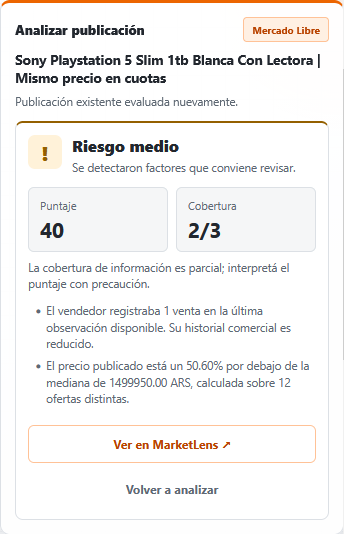
\includegraphics[height=0.52\textheight,keepaspectratio]{figuras/marketlens/extension_riesgo_70.png}
\caption{Resultado de evaluación de riesgo de la publicación 70 mediante la extensión de MarketLens}
\label{fig:ml-extension-70}
\end{figure}

Este caso permitió comprobar el funcionamiento conjunto de la
comparación automática de precios, la evaluación del historial comercial
y el cálculo del índice de riesgo.

No obstante, el resultado constituye una estimación basada en las reglas
definidas por MarketLens. La presencia de un precio anormalmente bajo y
un historial limitado no demuestra por sí sola que una publicación sea
fraudulenta.

\subsection{Alcance de los resultados}

Los índices calculados hasta esta etapa representan resultados
funcionales preliminares.

La generación correcta de una puntuación permite verificar que el
mecanismo de evaluación puede ejecutarse utilizando los datos
disponibles, pero no demuestra por sí sola la precisión del sistema para
identificar situaciones reales de fraude.

Para validar dicha capacidad será necesario disponer de casos
suficientemente representativos y contrastar los resultados obtenidos
con información que permita establecer criterios de referencia.

En consecuencia, los resultados actuales constituyen una primera
comprobación del funcionamiento técnico del motor de riesgo, mientras
que la evaluación integral de su desempeño y la ampliación de su
cobertura permanecen como actividades de desarrollo y validación.

\section{Resultados de implementación}

El desarrollo de MarketLens permitió implementar una primera versión
funcional de la arquitectura propuesta en el Marco Tecnológico,
integrando una aplicación web, una API REST, una base de datos
relacional y una extensión de navegador destinada a facilitar la
interacción con marketplaces digitales.

La implementación se realizó mediante una arquitectura cliente-servidor
en capas, utilizando Java y Spring Boot para el backend, PostgreSQL para
la persistencia de información y React con TypeScript para la interfaz
web.

\subsection{Backend y persistencia de datos}

Se desarrolló una API REST encargada de centralizar las operaciones
principales de la plataforma, incluyendo la gestión de publicaciones,
vendedores, autenticación de usuarios y evaluación de riesgo.

La utilización de PostgreSQL permitió incorporar persistencia de datos,
de manera que la información gestionada por el sistema pudiera
conservarse y consultarse posteriormente.

Durante el desarrollo se realizaron pruebas de comunicación con los
endpoints implementados, verificando el procesamiento de solicitudes
HTTP y la recuperación de información mediante respuestas estructuradas
en formato JSON.

Asimismo, se implementaron mecanismos de autenticación y protección de
recursos para controlar el acceso a las funcionalidades del sistema.

\subsection{Aplicación web}

Se desarrolló una aplicación web utilizando React y TypeScript,
conectada con los servicios del backend.

La interfaz permite acceder a las principales áreas funcionales de la
plataforma, incluyendo la autenticación, la consulta de publicaciones,
la gestión de vendedores y la visualización de información estadística
mediante un dashboard.

La integración entre frontend y backend permitió verificar la
comunicación entre ambos componentes y trasladar determinadas
operaciones, inicialmente probadas mediante herramientas de consulta de
APIs, a una interfaz gráfica.

\subsection{Extensión de navegador}

Se avanzó en el desarrollo de una extensión de navegador destinada a
permitir que los usuarios interactúen con MarketLens mientras consultan
publicaciones en plataformas externas.

Las pruebas iniciales se concentraron en Mercado Libre, donde se logró
extraer información de determinadas publicaciones y vendedores,
incluyendo atributos utilizados por el mecanismo de evaluación de
riesgo.

Este componente constituye un elemento importante de la solución, dado
que permite complementar la información obtenida mediante APIs externas
y facilita la incorporación de datos provenientes de publicaciones
consultadas directamente por los usuarios.

Los resultados obtenidos demuestran el funcionamiento inicial de la
comunicación entre los componentes de la arquitectura, aunque
determinadas integraciones y funcionalidades continúan en desarrollo.

\section{Resultados de integración}

La integración con plataformas externas constituye uno de los aspectos
más relevantes del desarrollo de MarketLens, debido a que la
disponibilidad y estructura de la información varía según el marketplace
y el tipo de publicación analizada.

Durante esta etapa se realizaron pruebas de integración con Mercado
Libre, utilizando tanto los servicios disponibles mediante su API como
los mecanismos de extracción de información incorporados a la extensión
de navegador.

\subsection{Integración mediante API}

Se realizaron pruebas de autenticación e interacción con los servicios
de Mercado Libre, logrando establecer una conexión autorizada y ejecutar
determinadas consultas.

Sin embargo, también se identificaron restricciones de acceso a algunos
recursos, especialmente en operaciones relacionadas con información de
terceros. Estas limitaciones evidenciaron que la disponibilidad de una
API no garantiza necesariamente el acceso a todos los atributos
requeridos por el sistema.

Ante esta situación, se continuó trabajando con la extensión de
navegador como mecanismo complementario de obtención de información, de
acuerdo con la arquitectura prevista.

\subsection{Extracción de información desde publicaciones}

Las pruebas realizadas con la extensión permitieron recuperar
determinados atributos de publicaciones y vendedores de Mercado Libre.

Entre los resultados obtenidos se encuentra la identificación de un
vendedor y la recuperación de información relacionada con su reputación.
Estos datos pudieron contrastarse mediante consultas a los servicios
externos disponibles.

No obstante, algunos atributos no estuvieron presentes en las respuestas
recibidas. Por ejemplo, la fecha de registro del vendedor no pudo
recuperarse en una de las pruebas, aun cuando sí se obtuvo información
sobre su identificación y reputación.

Esto permitió identificar la necesidad de manejar atributos opcionales o
no disponibles sin impedir innecesariamente el procesamiento del resto
de la información.

\subsection{Diferencias entre publicaciones individuales y publicaciones de catálogo}

Durante las pruebas se identificaron diferencias en el procesamiento de
publicaciones individuales y publicaciones de catálogo de Mercado Libre.

El sistema consiguió obtener información y realizar evaluaciones de
riesgo sobre determinadas publicaciones individuales. Sin embargo, el
tratamiento de publicaciones de catálogo todavía presenta dificultades
que impiden completar algunos análisis.

Esta situación requiere adaptar los mecanismos de identificación y
recuperación de información para contemplar las diferentes estructuras
de publicación utilizadas por la plataforma.

Por lo tanto, si bien se logró comprobar parcialmente la viabilidad de
la integración, todavía no puede afirmarse que el mecanismo desarrollado
sea compatible con todas las modalidades de publicación de Mercado
Libre.

La resolución de estas diferencias constituye una de las actividades
pendientes para ampliar la cobertura funcional de MarketLens.

\section{Pruebas funcionales y de integración}

\begin{table}[H]
\centering
\caption{Pruebas funcionales y de integración registradas}
\label{tab:ml-pruebas}
\scriptsize
\begin{tabularx}{\textwidth}{L L L L}
\toprule
\tb{Prueba} & \tb{Esperado} & \tb{Obtenido} & \tb{Estado} \\
\midrule
Creación de publicaciones & Persistencia correcta & Persistencia correcta & Evidencia pendiente \\
Precio inferior & 40/100, MEDIUM & 40/100, MEDIUM & Comprobación puntual \\
Referencia insuficiente & Sin penalización & Sin penalización & Comprobación puntual \\
Autenticación JWT & Acceso y rechazo correctos & Funcionamiento informado & Validación parcial \\
Evaluación desde extensión & Consistencia con backend & 40/100, publicación 70 & Comprobación puntual \\
\bottomrule
\end{tabularx}
\end{table}

Las pruebas presentadas corresponden a comprobaciones funcionales
realizadas durante el desarrollo del prototipo. Los casos identificados
como comprobados permitieron verificar el comportamiento esperado de
determinadas funcionalidades, mientras que aquellos con validación
parcial requieren la ejecución o documentación de escenarios
adicionales.

Como complemento de los resultados presentados, el \textbf{Apéndice C}
incluye registros representativos de las respuestas obtenidas mediante
los servicios \emph{REST} de \emph{MarketLens}, correspondientes al
análisis de precios y a las evaluaciones de riesgo de la publicación
\#70. Estos registros permiten observar los indicadores calculados y
documentar las modificaciones realizadas sobre las ponderaciones del
motor durante el desarrollo.

% Encuesta exploratoria incorporada a partir del corte del CSV.
%!TEX root = ../main.tex
% Generado del archivo CSV de Google Forms. Corte: 15/11/2026.
% Insertar desde capitulos/07-resultados.tex mediante %!TEX root = ../main.tex
% Generado del archivo CSV de Google Forms. Corte: 15/11/2026.
% Insertar desde capitulos/07-resultados.tex mediante %!TEX root = ../main.tex
% Generado del archivo CSV de Google Forms. Corte: 15/11/2026.
% Insertar desde capitulos/07-resultados.tex mediante \input{capitulos/07-resultados-encuesta}

\section{Resultados de la encuesta exploratoria}
\label{sec:ml-resultados-encuesta}

Con el propósito de explorar las percepciones de los compradores sobre la seguridad en plataformas digitales y el interés por herramientas preventivas, se aplicó un cuestionario de once preguntas cerradas. El corte de resultados analizado comprende \textbf{61 respuestas} registradas entre el \textbf{10 y el 15 de noviembre de 2026}. El instrumento, sus opciones y las condiciones del relevamiento se incluyen en el apéndice~\ref{apx:encuesta}; el procedimiento se describe en la sección~\ref{subsec:ml-encuesta-metodo}.

La encuesta se difundió mediante contactos del autor y constituye un \textbf{relevamiento exploratorio no probabilístico}. Las cifras expresan percepciones e intenciones declaradas del grupo consultado, sin representatividad estadística de la población general ni evidencia directa de eficacia del motor de detección de fraudes. Las preguntas de selección múltiple admitieron varias alternativas; sus porcentajes se calcularon sobre los 61 participantes y pueden sumar más del 100\,\%.

\begin{table}[H]
\centering
\caption{Síntesis de resultados de la encuesta exploratoria (n=61)}
\label{tab:ml-encuesta-principales}
\small
\begin{tabularx}{\textwidth}{L r r}
\toprule
\tb{Indicador declarado} & \tb{Respuestas} & \tb{Porcentaje} \\
\midrule
Encontró alguna publicación sospechosa & 44/61 & 72,1\,\% \\
Desistió de una compra por desconfianza & 47/61 & 77,0\,\% \\
Calificó la utilidad potencial con 4 o 5 (escala de 1 a 5) & 50/61 & 82,0\,\% \\
Consideraría utilizarla de forma frecuente o ante dudas & 58/61 & 95,1\,\% \\
Asignó 4 o 5 de confianza a los mecanismos actuales & 35/61 & 57,4\,\% \\
\bottomrule
\end{tabularx}
\end{table}

\subsection{Experiencia de compra y criterios de evaluación}

El cuestionario contempló tanto participantes que habían comprado durante los últimos doce meses como otros que no lo habían hecho. El uso de cada plataforma, que podía informarse en conjunto con otras, se presenta en la figura~\ref{fig:ml-encuesta-02}. Mercado Libre fue seleccionado por \textbf{52 personas (85,2\,\%)}. En cuanto a los criterios consultados, los más frecuentes fueron la reputación o calificaciones del vendedor (\textbf{50/61}) y las opiniones de compradores anteriores (\textbf{47/61}), tal como muestra la figura~\ref{fig:ml-encuesta-03}.

\subsection{Percepción de riesgo y confianza}

\textbf{44 participantes (72,1\,\%)} señalaron haber encontrado alguna publicación potencialmente sospechosa (figura~\ref{fig:ml-encuesta-04}), mientras que \textbf{47 (77,0\,\%)} indicaron haber desistido de una compra por desconfianza (figura~\ref{fig:ml-encuesta-05}). Ambas preguntas recogen experiencias autopercibidas: no identifican ni verifican casos reales de fraude.

La confianza en los mecanismos actuales de seguridad y reputación se distribuyó en la escala de 1 a 5, con 35 respuestas en los valores 4 o 5 (\textbf{57,4\,\%}). Entre las características que generaron mayor desconfianza se destacaron el precio considerablemente inferior al de ofertas comparables (\textbf{38 respuestas}), la ausencia de calificaciones u opiniones (\textbf{37}) y la solicitud de pago fuera de la plataforma (\textbf{35}). Se trata de percepciones de los participantes y no de una validación de esos indicadores como predictores de fraude.

\subsection{Utilidad percibida e intención declarada de uso}

Tras presentar una descripción conceptual de una herramienta independiente de análisis preventivo, \textbf{50 participantes (82,0\,\%)} asignaron una utilidad de 4 o 5 en una escala de cinco puntos (figura~\ref{fig:ml-encuesta-08}). Además, \textbf{58 (95,1\,\%)} manifestaron que probablemente utilizarían una herramienta gratuita con frecuencia o ante publicaciones que les generaran dudas (figura~\ref{fig:ml-encuesta-09}). Estas respuestas sugieren \emph{interés declarado} y no constituyen evidencia de adopción efectiva.

En cuanto a funcionalidades, la opción más señalada fue la información sobre el historial comercial del vendedor (\textbf{36 respuestas; 59,0\,\%}). Las advertencias sobre datos insuficientes y la explicación de los factores de riesgo reunieron 26 selecciones cada una. Entre las preocupaciones, destacaron la recopilación innecesaria de datos personales (\textbf{33 respuestas}), la información desactualizada (\textbf{30}) y las advertencias incorrectas (\textbf{26}). Estos resultados sirven para orientar prioridades de transparencia, privacidad y calidad de datos, pero por sí solos no validan decisiones técnicas específicas.

\subsection{Alcance y limitaciones del relevamiento}

La distribución del formulario entre contactos y la participación voluntaria introducen posibles \textbf{sesgos de selección y autoselección}. El instrumento no relevó variables sociodemográficas ni verificó en forma independiente las experiencias declaradas. Por consiguiente, no es posible generalizar los resultados a la totalidad de compradores ni estimar márgenes de error de muestreo probabilístico. Asimismo, la descripción conceptual de MarketLens puede influir en las valoraciones de utilidad e intención de uso.

Estas evidencias complementan la justificación del problema abordado y permiten identificar prioridades expresadas por las personas encuestadas. No deben confundirse con pruebas de usabilidad del prototipo, validaciones de precisión del índice de riesgo o una medición de su impacto real en la prevención de estafas. El presente corte corresponde a 61 respuestas; de incorporarse nuevas respuestas, deben recalcularse todos los porcentajes y sustituirse los gráficos correspondientes.

\subsection{Distribución completa de respuestas}

Las figuras siguientes presentan las frecuencias absolutas y los porcentajes observados para las once preguntas, incluida la opción de valoración no seleccionada en las escalas. En preguntas de selección múltiple, el denominador continúa siendo el número total de participantes (61).
\begin{figure}[H]
\centering
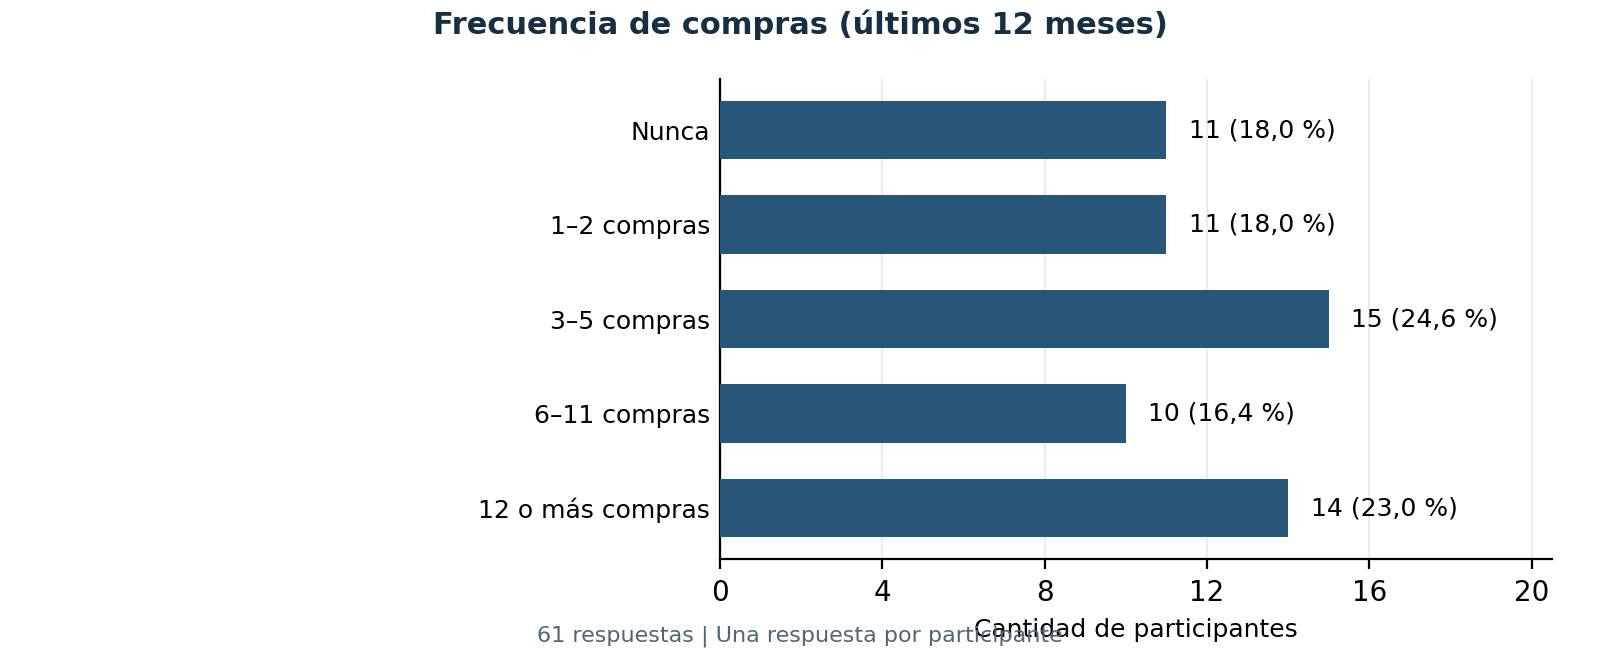
\includegraphics[width=0.94\textwidth,height=0.37\textheight,keepaspectratio]{figuras/marketlens/encuesta/pregunta_01.png}
\caption{Frecuencia de compra declarada en marketplaces durante los últimos doce meses (n=61).}\label{fig:ml-encuesta-01}
\end{figure}

\begin{figure}[H]
\centering
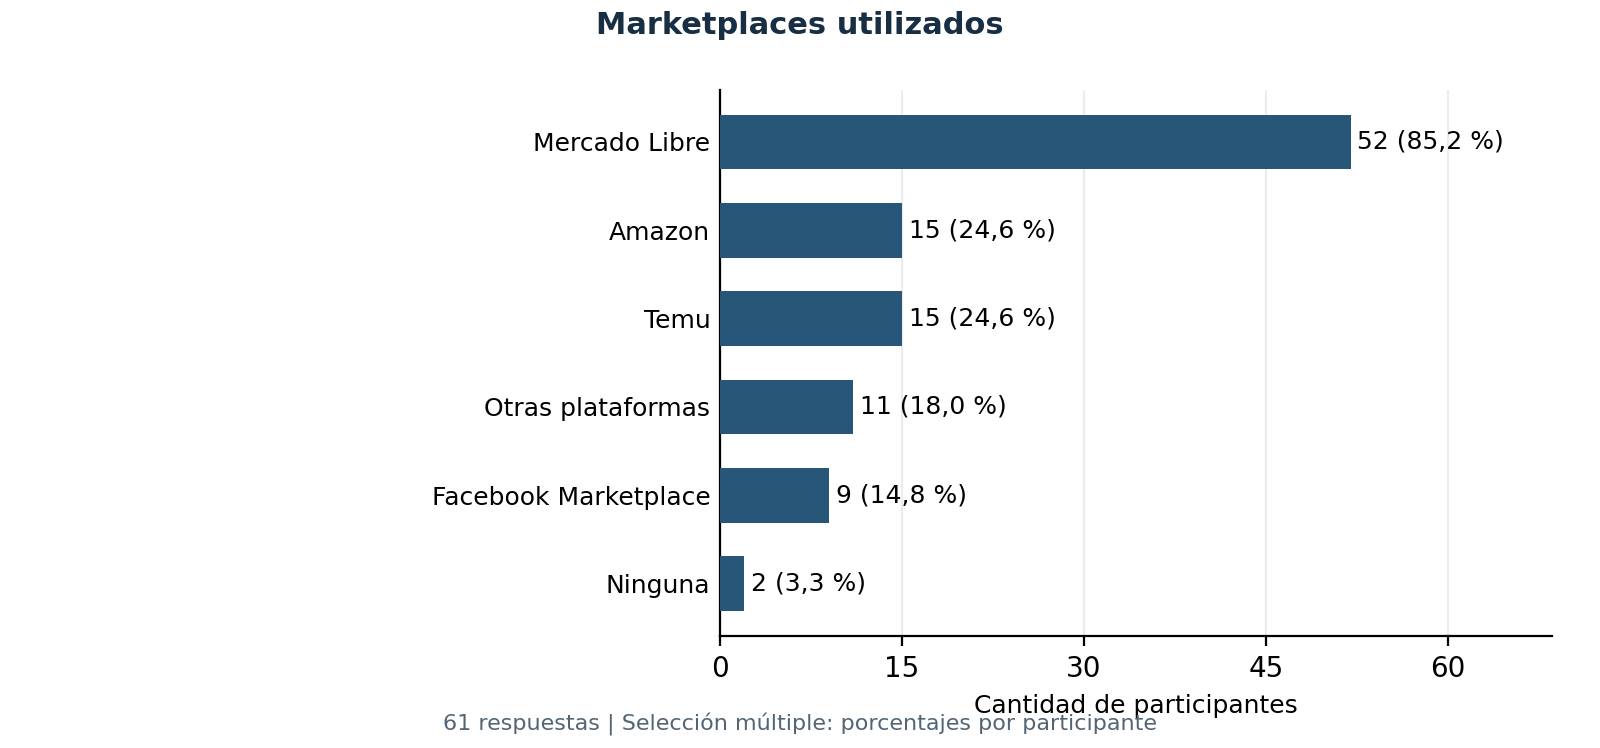
\includegraphics[width=0.94\textwidth,height=0.37\textheight,keepaspectratio]{figuras/marketlens/encuesta/pregunta_02.png}
\caption{Plataformas utilizadas por los encuestados durante los últimos doce meses (n=61).}\label{fig:ml-encuesta-02}
\end{figure}

\begin{figure}[H]
\centering
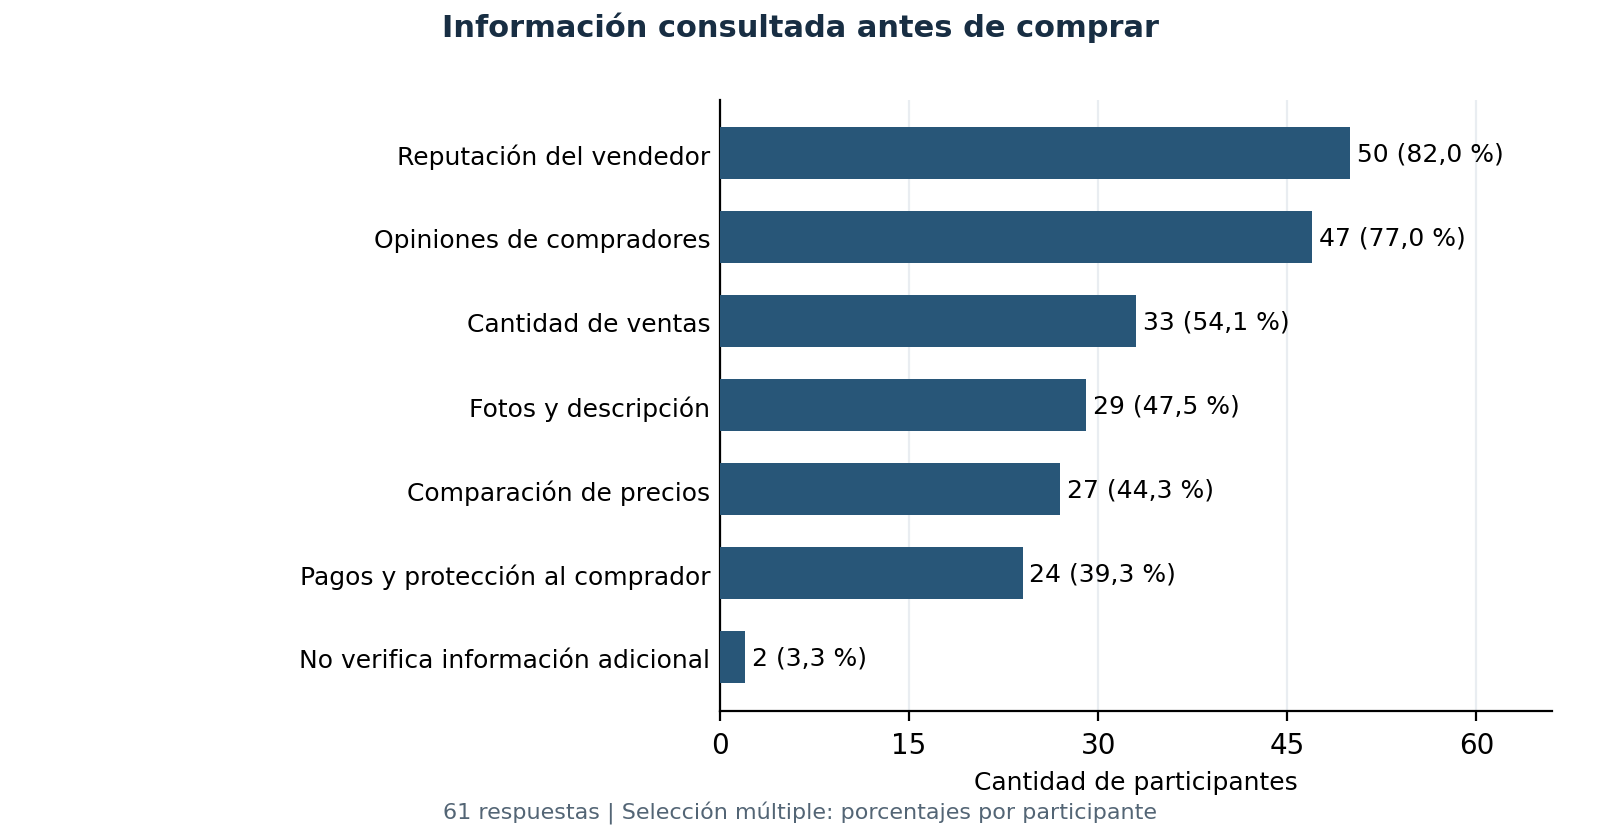
\includegraphics[width=0.94\textwidth,height=0.37\textheight,keepaspectratio]{figuras/marketlens/encuesta/pregunta_03.png}
\caption{Información habitualmente consultada para evaluar publicaciones o vendedores (n=61).}\label{fig:ml-encuesta-03}
\end{figure}

\begin{figure}[H]
\centering
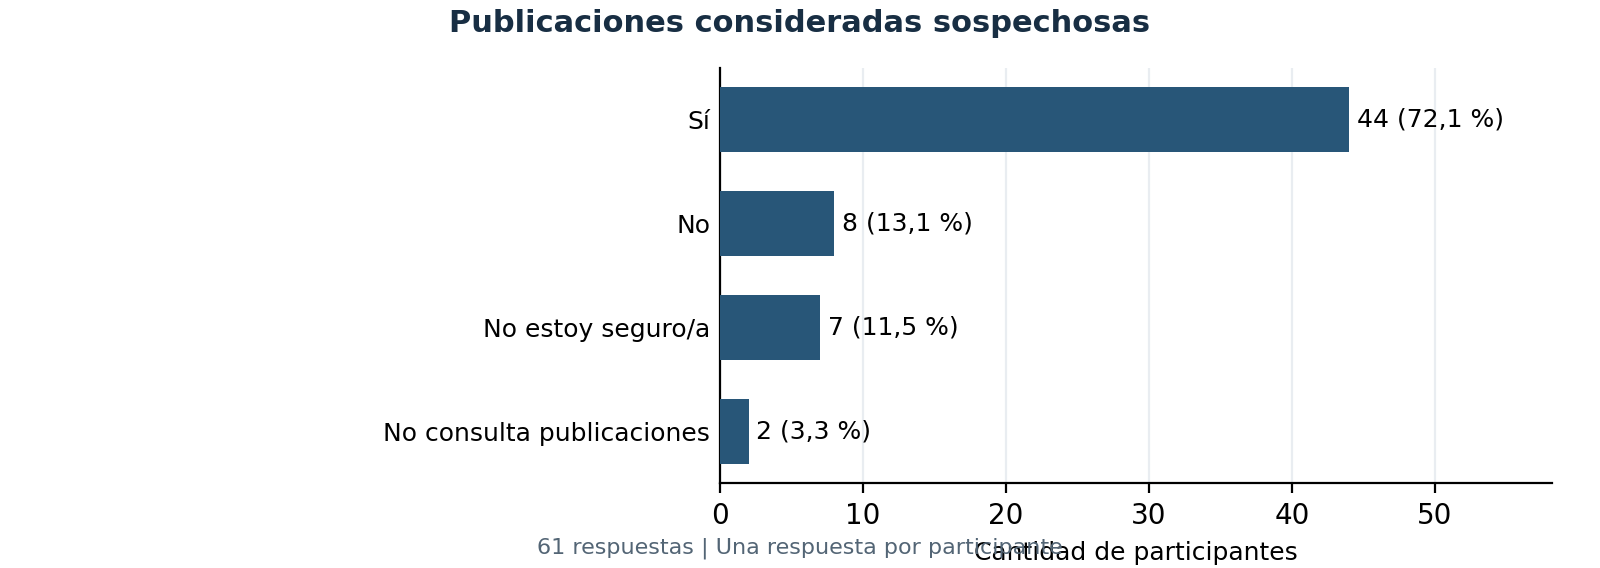
\includegraphics[width=0.94\textwidth,height=0.37\textheight,keepaspectratio]{figuras/marketlens/encuesta/pregunta_04.png}
\caption{Encuestados que identificaron publicaciones potencialmente sospechosas (n=61).}\label{fig:ml-encuesta-04}
\end{figure}

\begin{figure}[H]
\centering
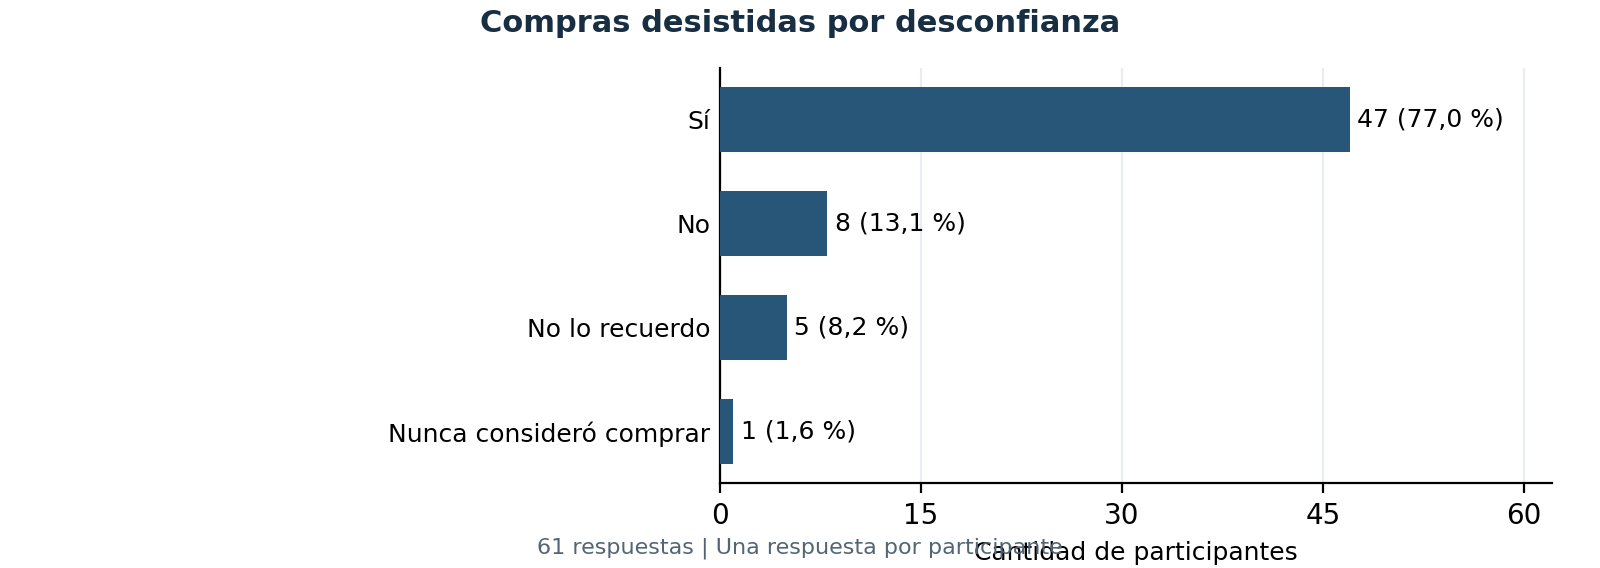
\includegraphics[width=0.94\textwidth,height=0.37\textheight,keepaspectratio]{figuras/marketlens/encuesta/pregunta_05.png}
\caption{Encuestados que desistieron de una compra por desconfianza (n=61).}\label{fig:ml-encuesta-05}
\end{figure}

\begin{figure}[H]
\centering
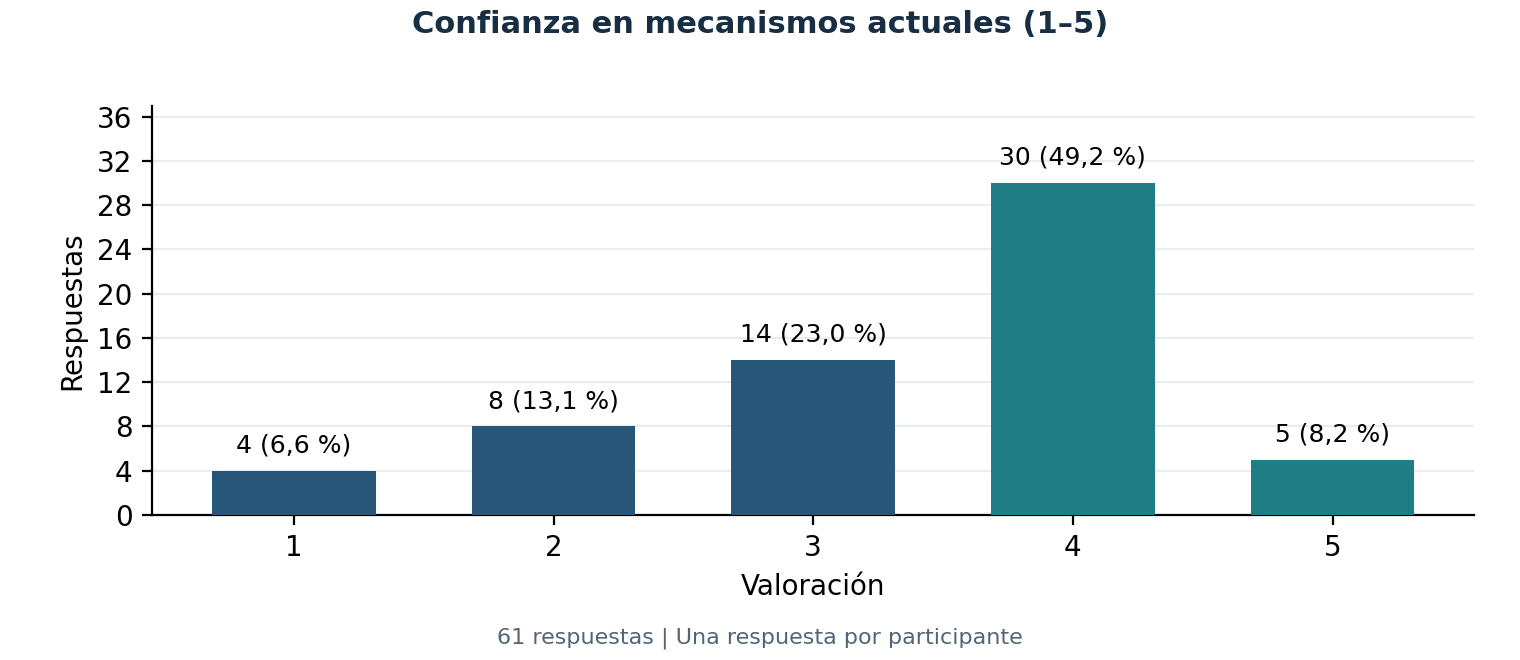
\includegraphics[width=0.94\textwidth,height=0.37\textheight,keepaspectratio]{figuras/marketlens/encuesta/pregunta_06.png}
\caption{Confianza declarada en los mecanismos actuales de seguridad y reputación (n=61).}\label{fig:ml-encuesta-06}
\end{figure}

\begin{figure}[H]
\centering
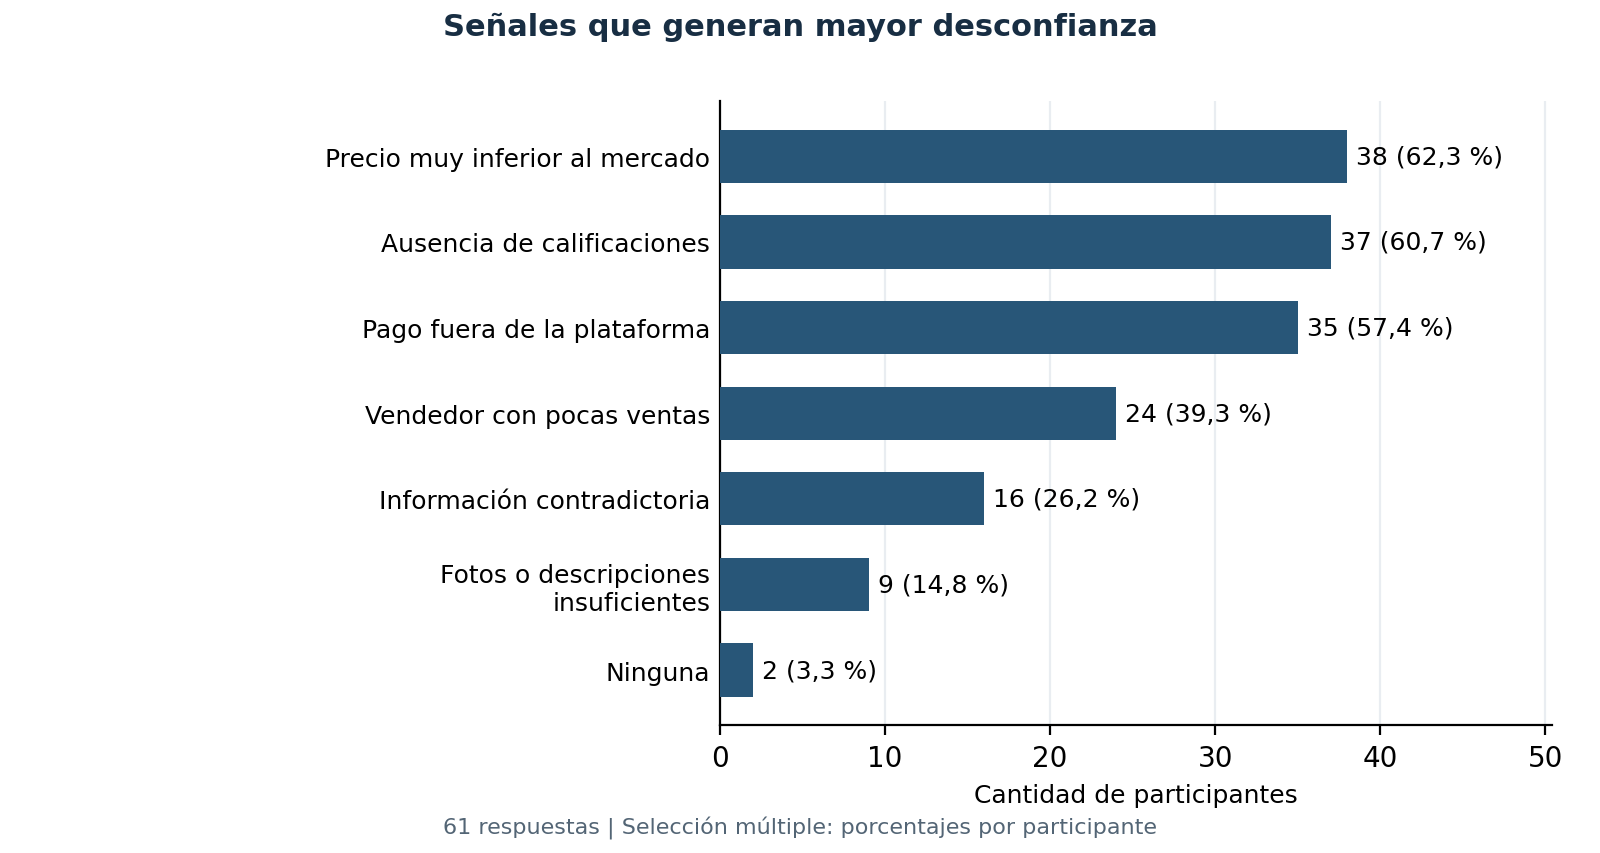
\includegraphics[width=0.94\textwidth,height=0.37\textheight,keepaspectratio]{figuras/marketlens/encuesta/pregunta_07.png}
\caption{Características de publicaciones que generan mayor desconfianza (n=61).}\label{fig:ml-encuesta-07}
\end{figure}

\begin{figure}[H]
\centering
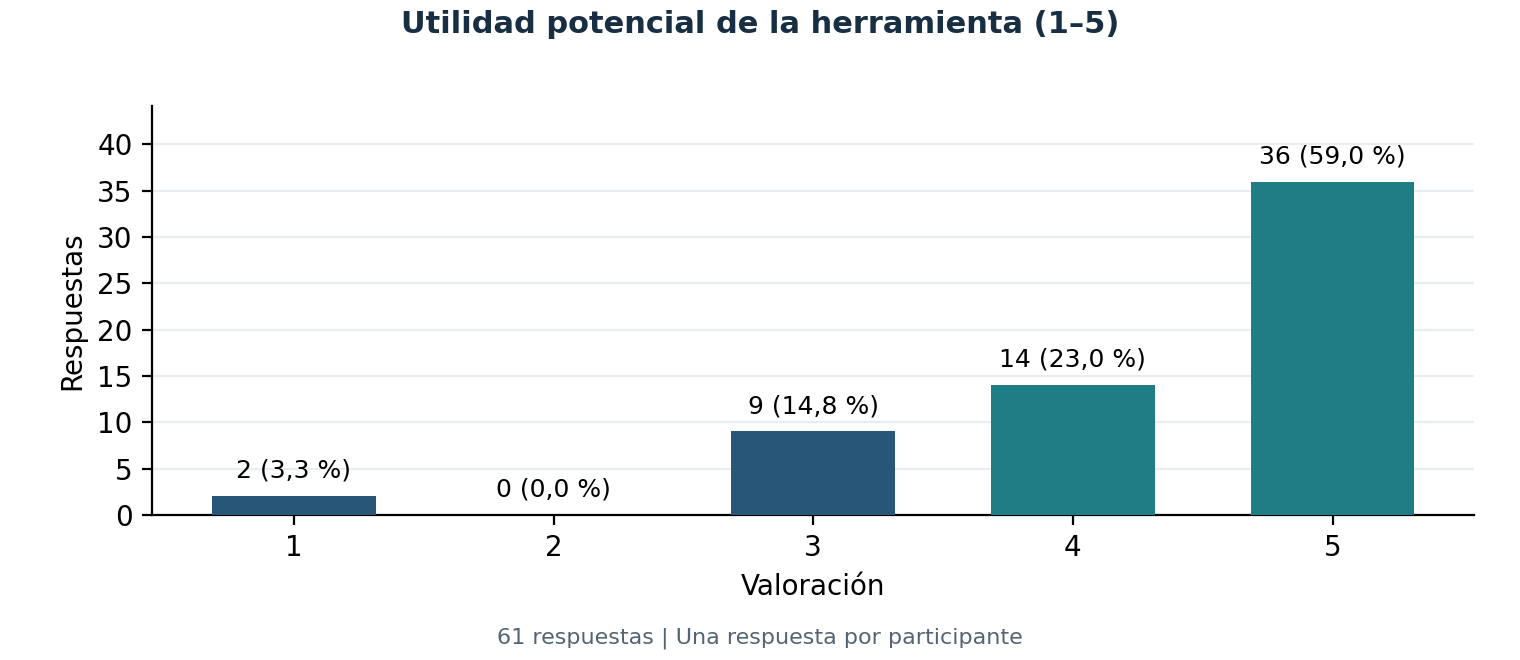
\includegraphics[width=0.94\textwidth,height=0.37\textheight,keepaspectratio]{figuras/marketlens/encuesta/pregunta_08.png}
\caption{Utilidad potencial atribuida a una herramienta de análisis preventivo (n=61).}\label{fig:ml-encuesta-08}
\end{figure}

\begin{figure}[H]
\centering
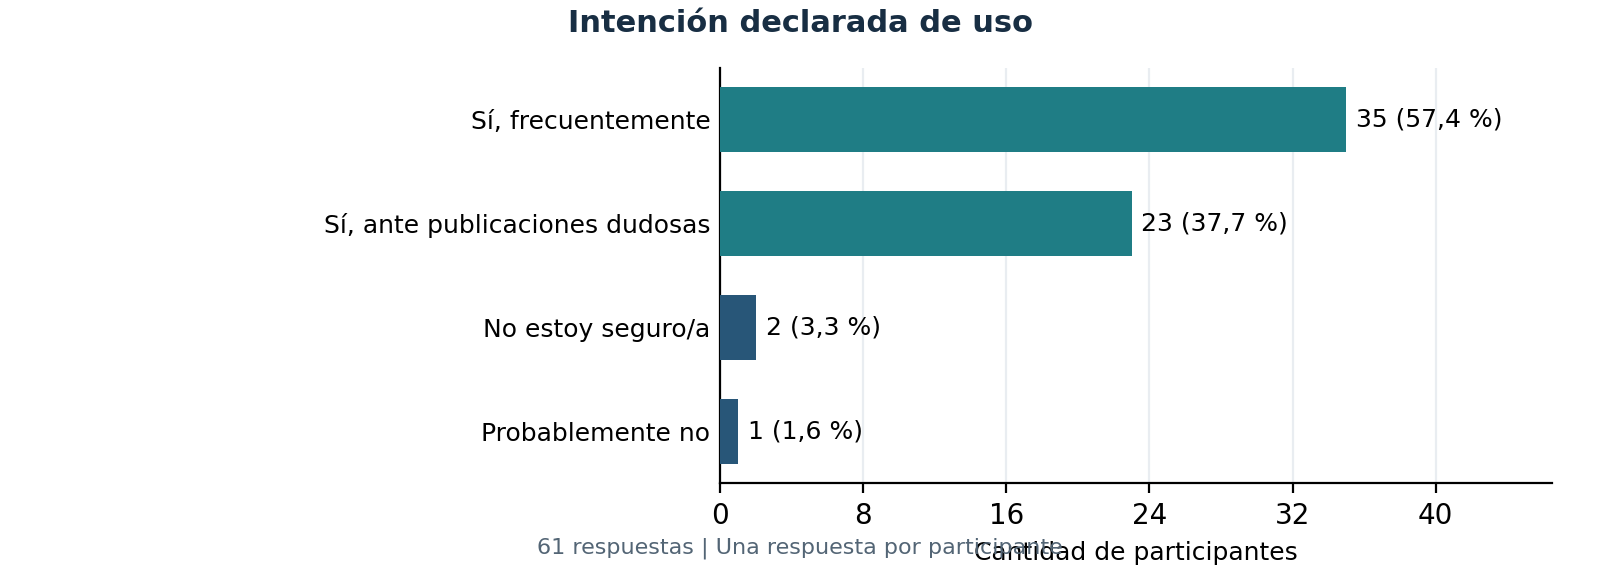
\includegraphics[width=0.94\textwidth,height=0.37\textheight,keepaspectratio]{figuras/marketlens/encuesta/pregunta_09.png}
\caption{Intención declarada de utilización de una herramienta gratuita como la propuesta (n=61).}\label{fig:ml-encuesta-09}
\end{figure}

\begin{figure}[H]
\centering
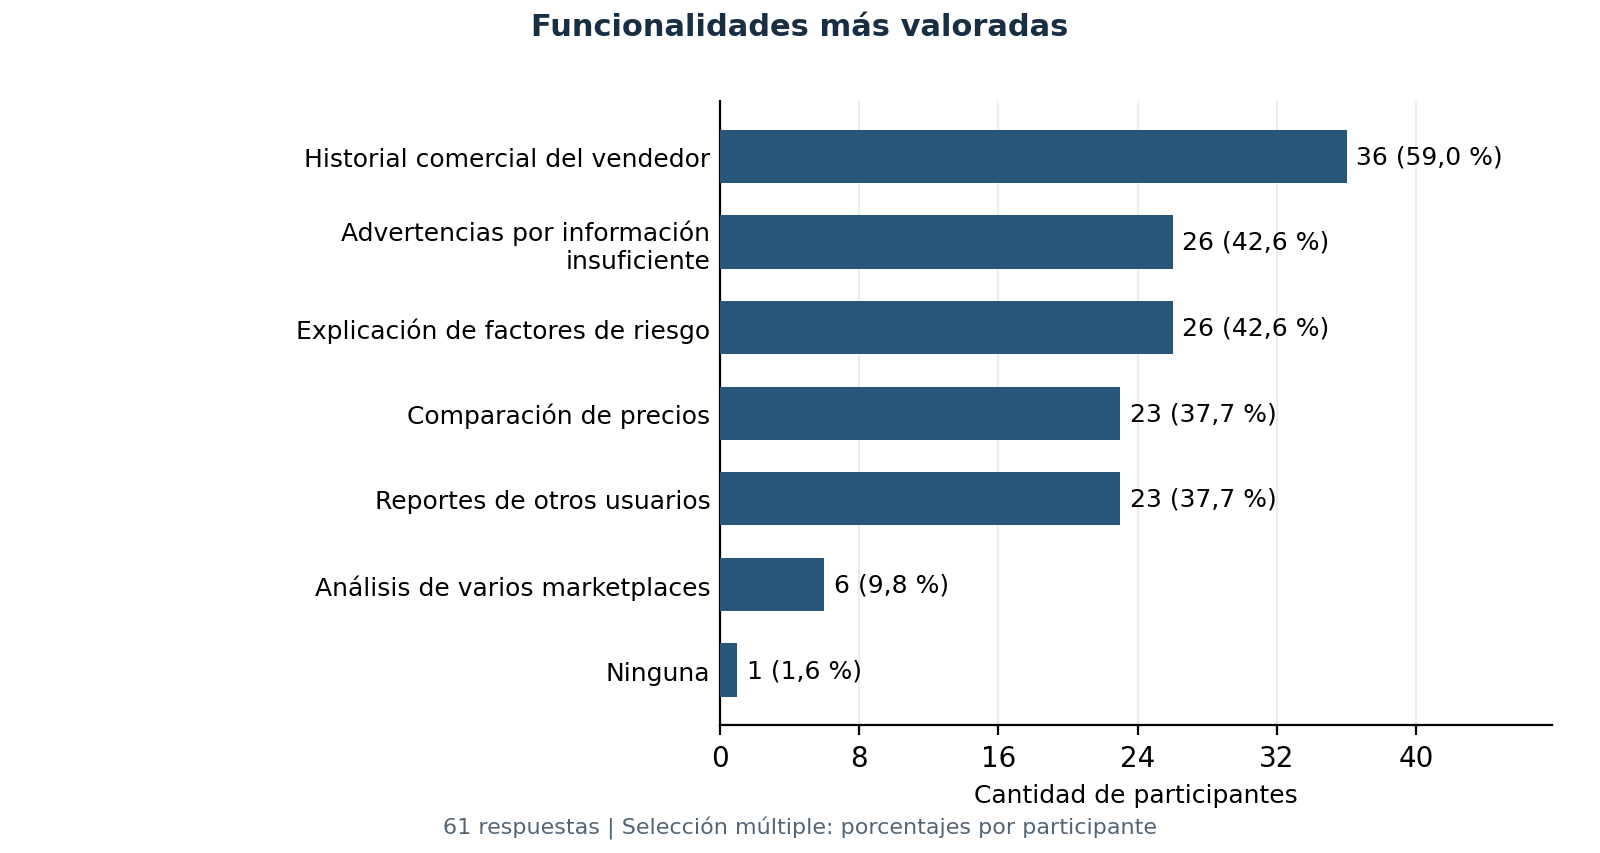
\includegraphics[width=0.94\textwidth,height=0.37\textheight,keepaspectratio]{figuras/marketlens/encuesta/pregunta_10.png}
\caption{Funcionalidades prioritarias para una herramienta de análisis preventivo (n=61).}\label{fig:ml-encuesta-10}
\end{figure}

\begin{figure}[H]
\centering
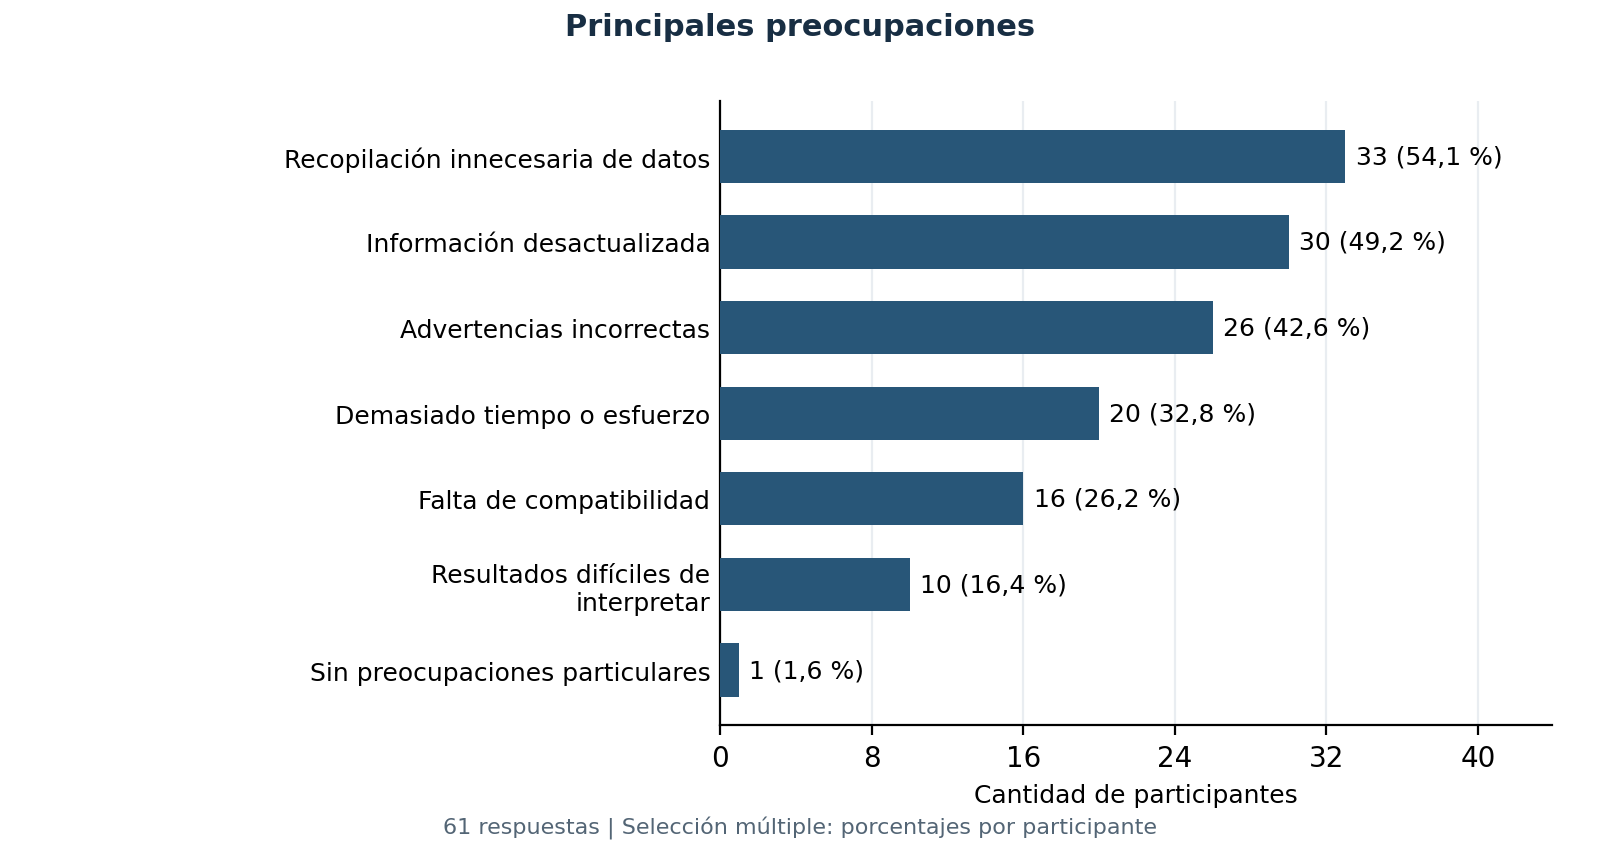
\includegraphics[width=0.94\textwidth,height=0.37\textheight,keepaspectratio]{figuras/marketlens/encuesta/pregunta_11.png}
\caption{Principales preocupaciones respecto del uso de la herramienta (n=61).}\label{fig:ml-encuesta-11}
\end{figure}



\section{Resultados de la encuesta exploratoria}
\label{sec:ml-resultados-encuesta}

Con el propósito de explorar las percepciones de los compradores sobre la seguridad en plataformas digitales y el interés por herramientas preventivas, se aplicó un cuestionario de once preguntas cerradas. El corte de resultados analizado comprende \textbf{61 respuestas} registradas entre el \textbf{10 y el 15 de noviembre de 2026}. El instrumento, sus opciones y las condiciones del relevamiento se incluyen en el apéndice~\ref{apx:encuesta}; el procedimiento se describe en la sección~\ref{subsec:ml-encuesta-metodo}.

La encuesta se difundió mediante contactos del autor y constituye un \textbf{relevamiento exploratorio no probabilístico}. Las cifras expresan percepciones e intenciones declaradas del grupo consultado, sin representatividad estadística de la población general ni evidencia directa de eficacia del motor de detección de fraudes. Las preguntas de selección múltiple admitieron varias alternativas; sus porcentajes se calcularon sobre los 61 participantes y pueden sumar más del 100\,\%.

\begin{table}[H]
\centering
\caption{Síntesis de resultados de la encuesta exploratoria (n=61)}
\label{tab:ml-encuesta-principales}
\small
\begin{tabularx}{\textwidth}{L r r}
\toprule
\tb{Indicador declarado} & \tb{Respuestas} & \tb{Porcentaje} \\
\midrule
Encontró alguna publicación sospechosa & 44/61 & 72,1\,\% \\
Desistió de una compra por desconfianza & 47/61 & 77,0\,\% \\
Calificó la utilidad potencial con 4 o 5 (escala de 1 a 5) & 50/61 & 82,0\,\% \\
Consideraría utilizarla de forma frecuente o ante dudas & 58/61 & 95,1\,\% \\
Asignó 4 o 5 de confianza a los mecanismos actuales & 35/61 & 57,4\,\% \\
\bottomrule
\end{tabularx}
\end{table}

\subsection{Experiencia de compra y criterios de evaluación}

El cuestionario contempló tanto participantes que habían comprado durante los últimos doce meses como otros que no lo habían hecho. El uso de cada plataforma, que podía informarse en conjunto con otras, se presenta en la figura~\ref{fig:ml-encuesta-02}. Mercado Libre fue seleccionado por \textbf{52 personas (85,2\,\%)}. En cuanto a los criterios consultados, los más frecuentes fueron la reputación o calificaciones del vendedor (\textbf{50/61}) y las opiniones de compradores anteriores (\textbf{47/61}), tal como muestra la figura~\ref{fig:ml-encuesta-03}.

\subsection{Percepción de riesgo y confianza}

\textbf{44 participantes (72,1\,\%)} señalaron haber encontrado alguna publicación potencialmente sospechosa (figura~\ref{fig:ml-encuesta-04}), mientras que \textbf{47 (77,0\,\%)} indicaron haber desistido de una compra por desconfianza (figura~\ref{fig:ml-encuesta-05}). Ambas preguntas recogen experiencias autopercibidas: no identifican ni verifican casos reales de fraude.

La confianza en los mecanismos actuales de seguridad y reputación se distribuyó en la escala de 1 a 5, con 35 respuestas en los valores 4 o 5 (\textbf{57,4\,\%}). Entre las características que generaron mayor desconfianza se destacaron el precio considerablemente inferior al de ofertas comparables (\textbf{38 respuestas}), la ausencia de calificaciones u opiniones (\textbf{37}) y la solicitud de pago fuera de la plataforma (\textbf{35}). Se trata de percepciones de los participantes y no de una validación de esos indicadores como predictores de fraude.

\subsection{Utilidad percibida e intención declarada de uso}

Tras presentar una descripción conceptual de una herramienta independiente de análisis preventivo, \textbf{50 participantes (82,0\,\%)} asignaron una utilidad de 4 o 5 en una escala de cinco puntos (figura~\ref{fig:ml-encuesta-08}). Además, \textbf{58 (95,1\,\%)} manifestaron que probablemente utilizarían una herramienta gratuita con frecuencia o ante publicaciones que les generaran dudas (figura~\ref{fig:ml-encuesta-09}). Estas respuestas sugieren \emph{interés declarado} y no constituyen evidencia de adopción efectiva.

En cuanto a funcionalidades, la opción más señalada fue la información sobre el historial comercial del vendedor (\textbf{36 respuestas; 59,0\,\%}). Las advertencias sobre datos insuficientes y la explicación de los factores de riesgo reunieron 26 selecciones cada una. Entre las preocupaciones, destacaron la recopilación innecesaria de datos personales (\textbf{33 respuestas}), la información desactualizada (\textbf{30}) y las advertencias incorrectas (\textbf{26}). Estos resultados sirven para orientar prioridades de transparencia, privacidad y calidad de datos, pero por sí solos no validan decisiones técnicas específicas.

\subsection{Alcance y limitaciones del relevamiento}

La distribución del formulario entre contactos y la participación voluntaria introducen posibles \textbf{sesgos de selección y autoselección}. El instrumento no relevó variables sociodemográficas ni verificó en forma independiente las experiencias declaradas. Por consiguiente, no es posible generalizar los resultados a la totalidad de compradores ni estimar márgenes de error de muestreo probabilístico. Asimismo, la descripción conceptual de MarketLens puede influir en las valoraciones de utilidad e intención de uso.

Estas evidencias complementan la justificación del problema abordado y permiten identificar prioridades expresadas por las personas encuestadas. No deben confundirse con pruebas de usabilidad del prototipo, validaciones de precisión del índice de riesgo o una medición de su impacto real en la prevención de estafas. El presente corte corresponde a 61 respuestas; de incorporarse nuevas respuestas, deben recalcularse todos los porcentajes y sustituirse los gráficos correspondientes.

\subsection{Distribución completa de respuestas}

Las figuras siguientes presentan las frecuencias absolutas y los porcentajes observados para las once preguntas, incluida la opción de valoración no seleccionada en las escalas. En preguntas de selección múltiple, el denominador continúa siendo el número total de participantes (61).
\begin{figure}[H]
\centering
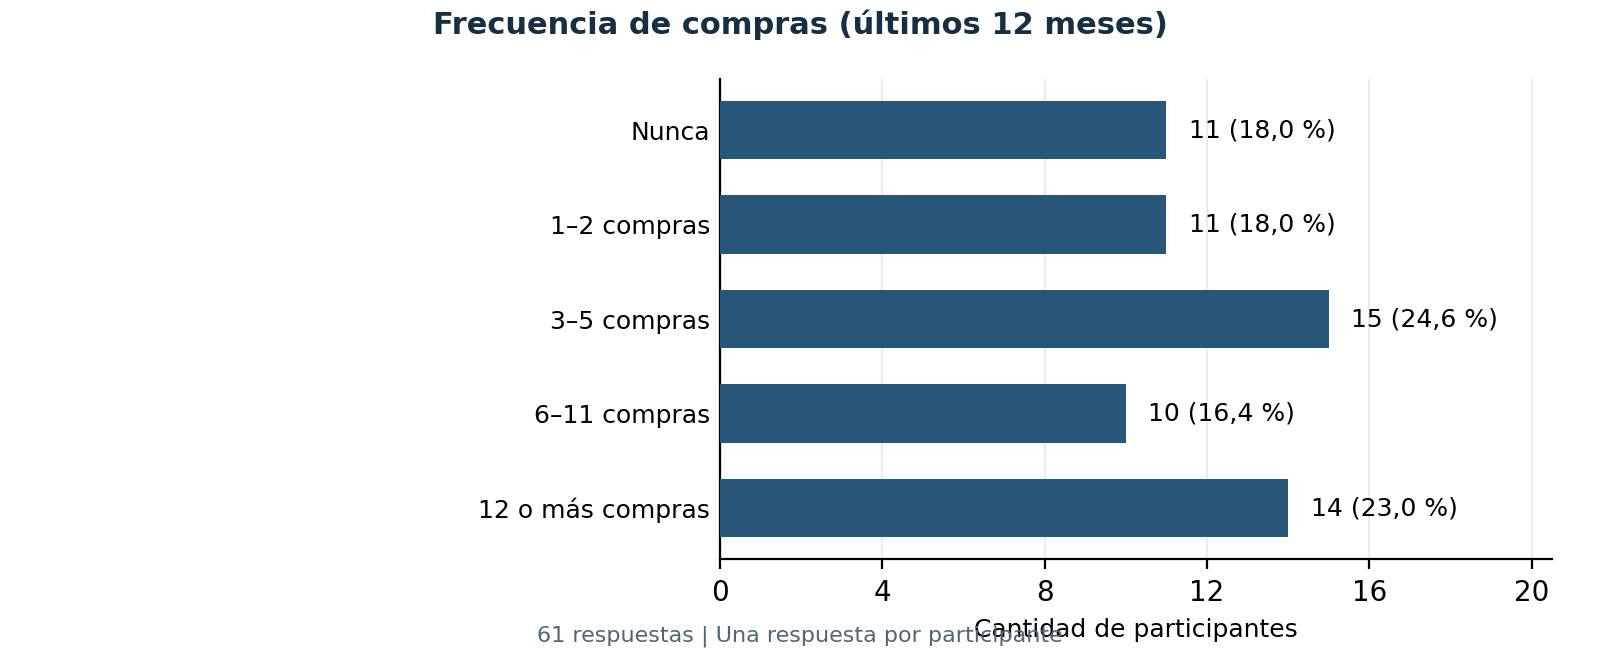
\includegraphics[width=0.94\textwidth,height=0.37\textheight,keepaspectratio]{figuras/marketlens/encuesta/pregunta_01.png}
\caption{Frecuencia de compra declarada en marketplaces durante los últimos doce meses (n=61).}\label{fig:ml-encuesta-01}
\end{figure}

\begin{figure}[H]
\centering
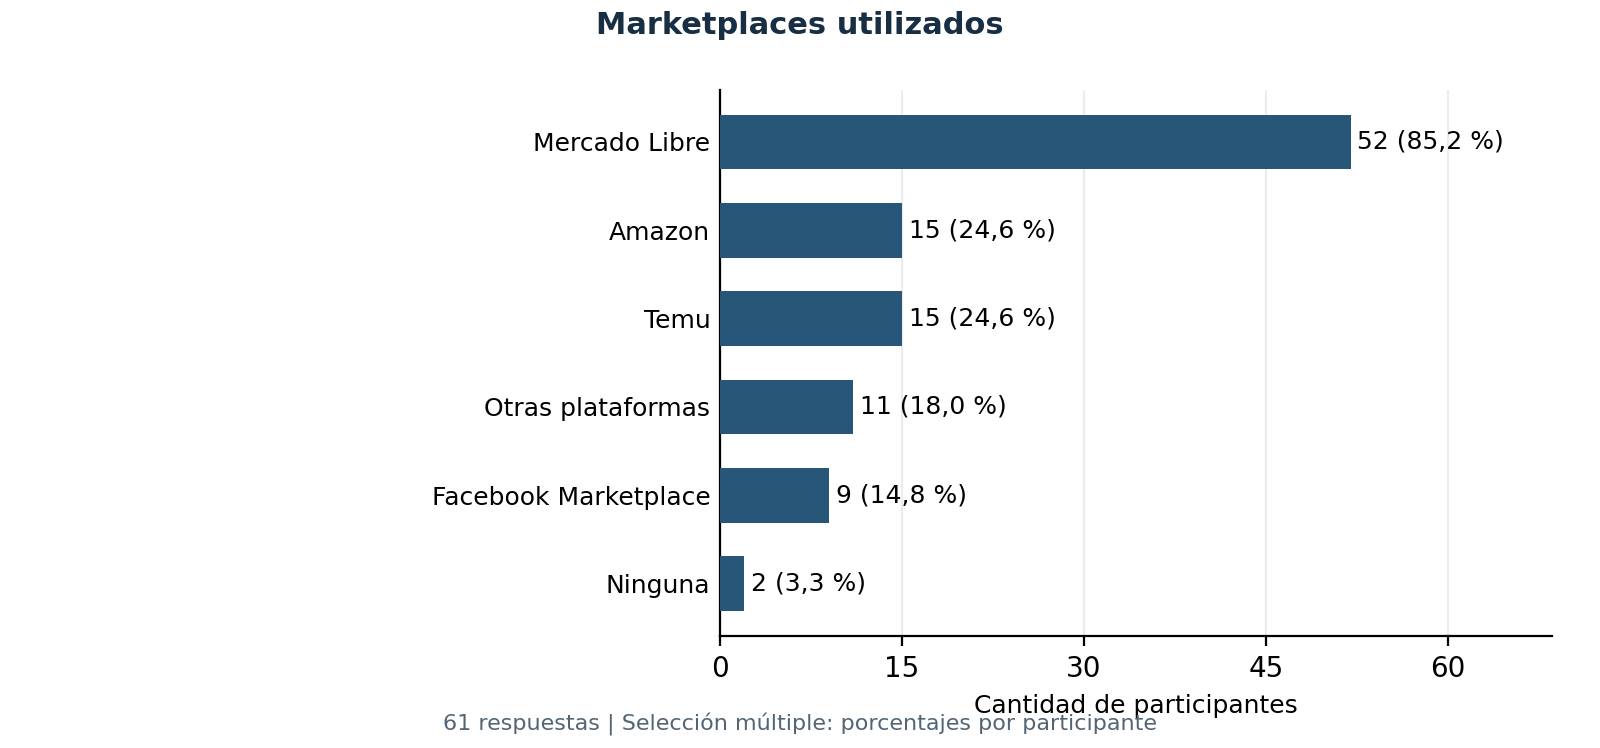
\includegraphics[width=0.94\textwidth,height=0.37\textheight,keepaspectratio]{figuras/marketlens/encuesta/pregunta_02.png}
\caption{Plataformas utilizadas por los encuestados durante los últimos doce meses (n=61).}\label{fig:ml-encuesta-02}
\end{figure}

\begin{figure}[H]
\centering
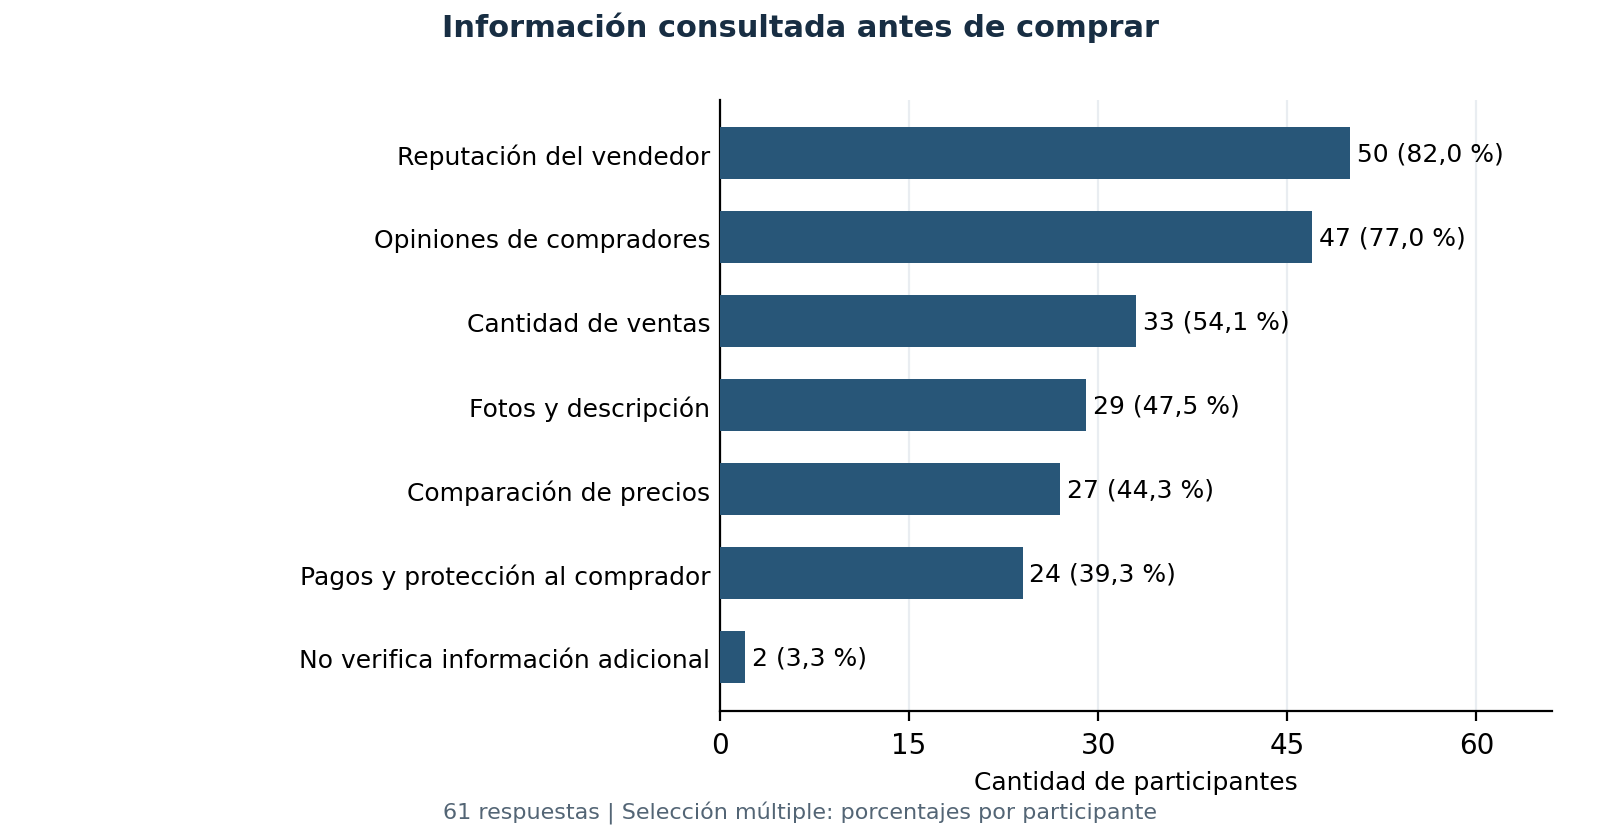
\includegraphics[width=0.94\textwidth,height=0.37\textheight,keepaspectratio]{figuras/marketlens/encuesta/pregunta_03.png}
\caption{Información habitualmente consultada para evaluar publicaciones o vendedores (n=61).}\label{fig:ml-encuesta-03}
\end{figure}

\begin{figure}[H]
\centering
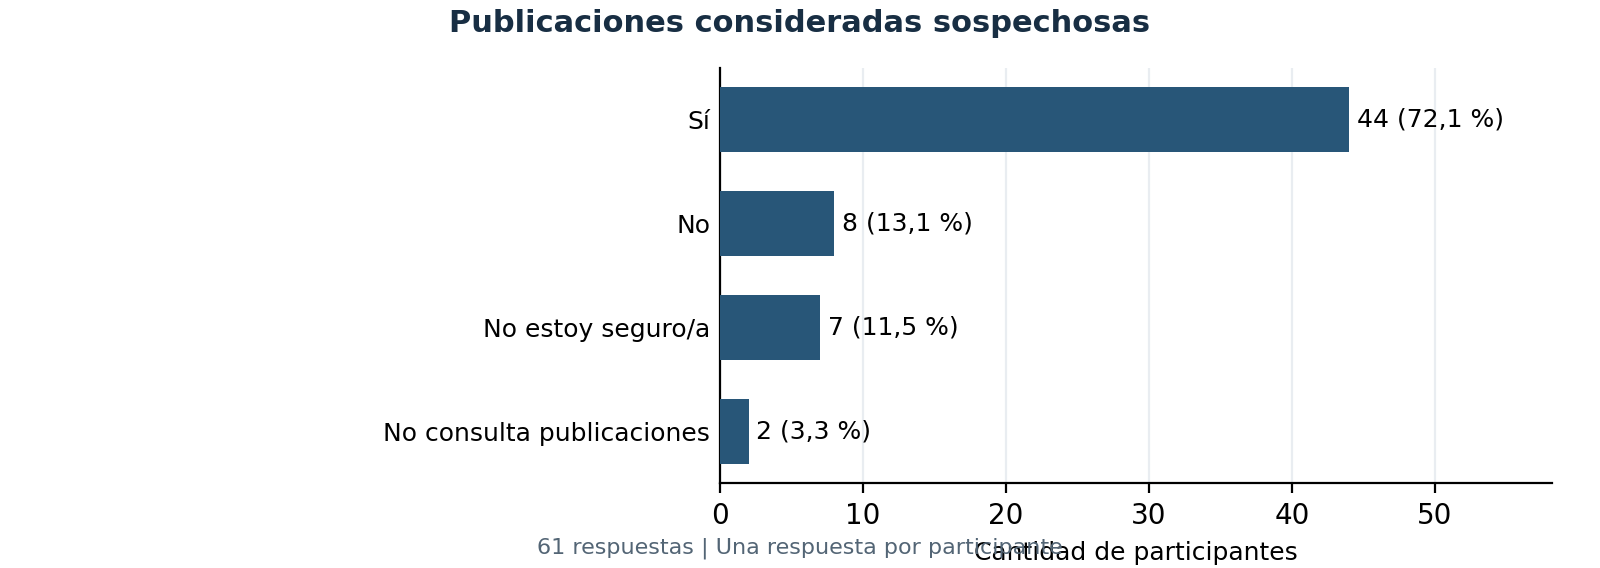
\includegraphics[width=0.94\textwidth,height=0.37\textheight,keepaspectratio]{figuras/marketlens/encuesta/pregunta_04.png}
\caption{Encuestados que identificaron publicaciones potencialmente sospechosas (n=61).}\label{fig:ml-encuesta-04}
\end{figure}

\begin{figure}[H]
\centering
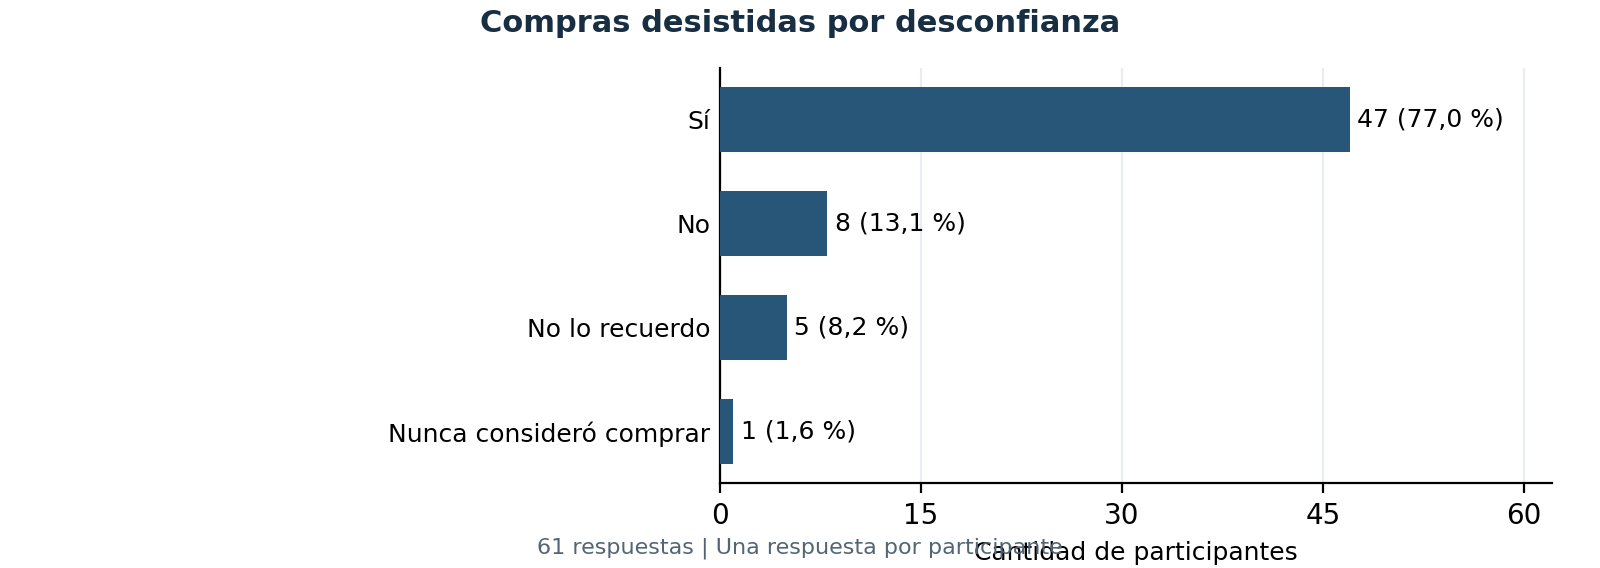
\includegraphics[width=0.94\textwidth,height=0.37\textheight,keepaspectratio]{figuras/marketlens/encuesta/pregunta_05.png}
\caption{Encuestados que desistieron de una compra por desconfianza (n=61).}\label{fig:ml-encuesta-05}
\end{figure}

\begin{figure}[H]
\centering
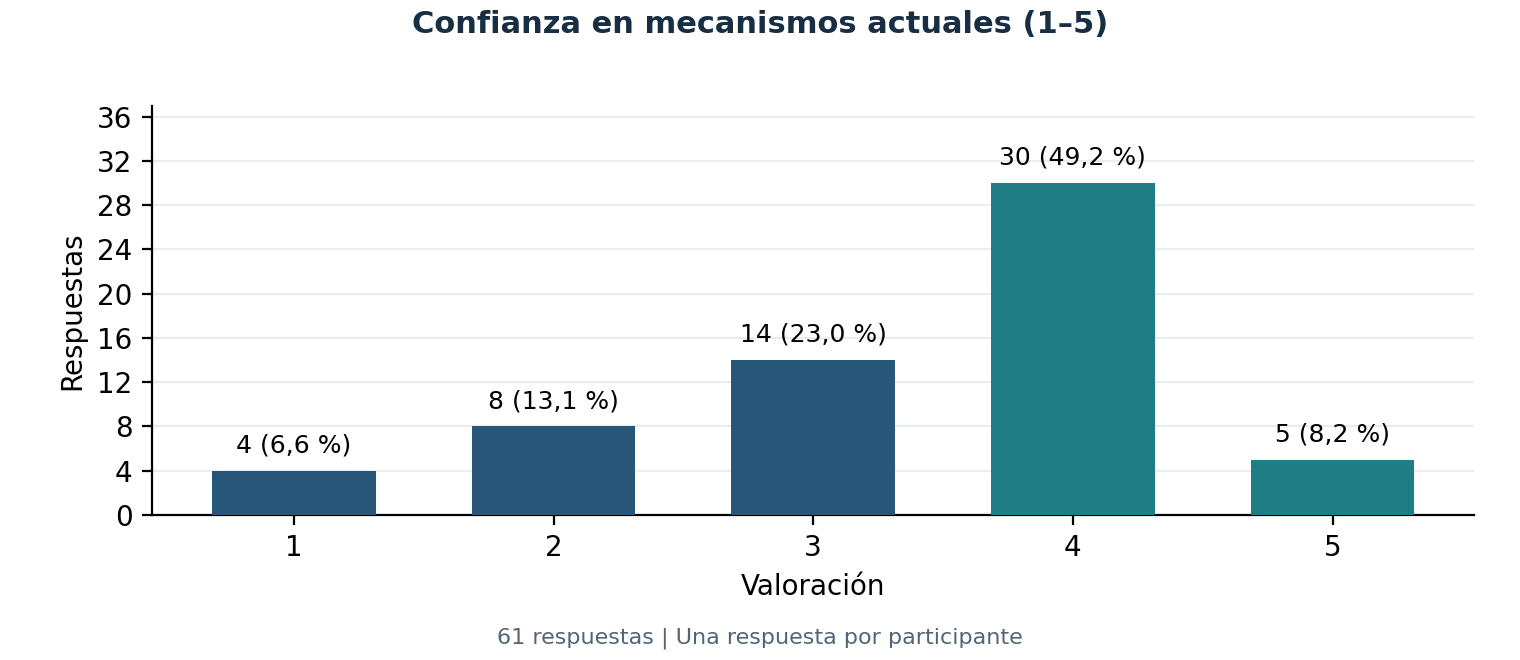
\includegraphics[width=0.94\textwidth,height=0.37\textheight,keepaspectratio]{figuras/marketlens/encuesta/pregunta_06.png}
\caption{Confianza declarada en los mecanismos actuales de seguridad y reputación (n=61).}\label{fig:ml-encuesta-06}
\end{figure}

\begin{figure}[H]
\centering
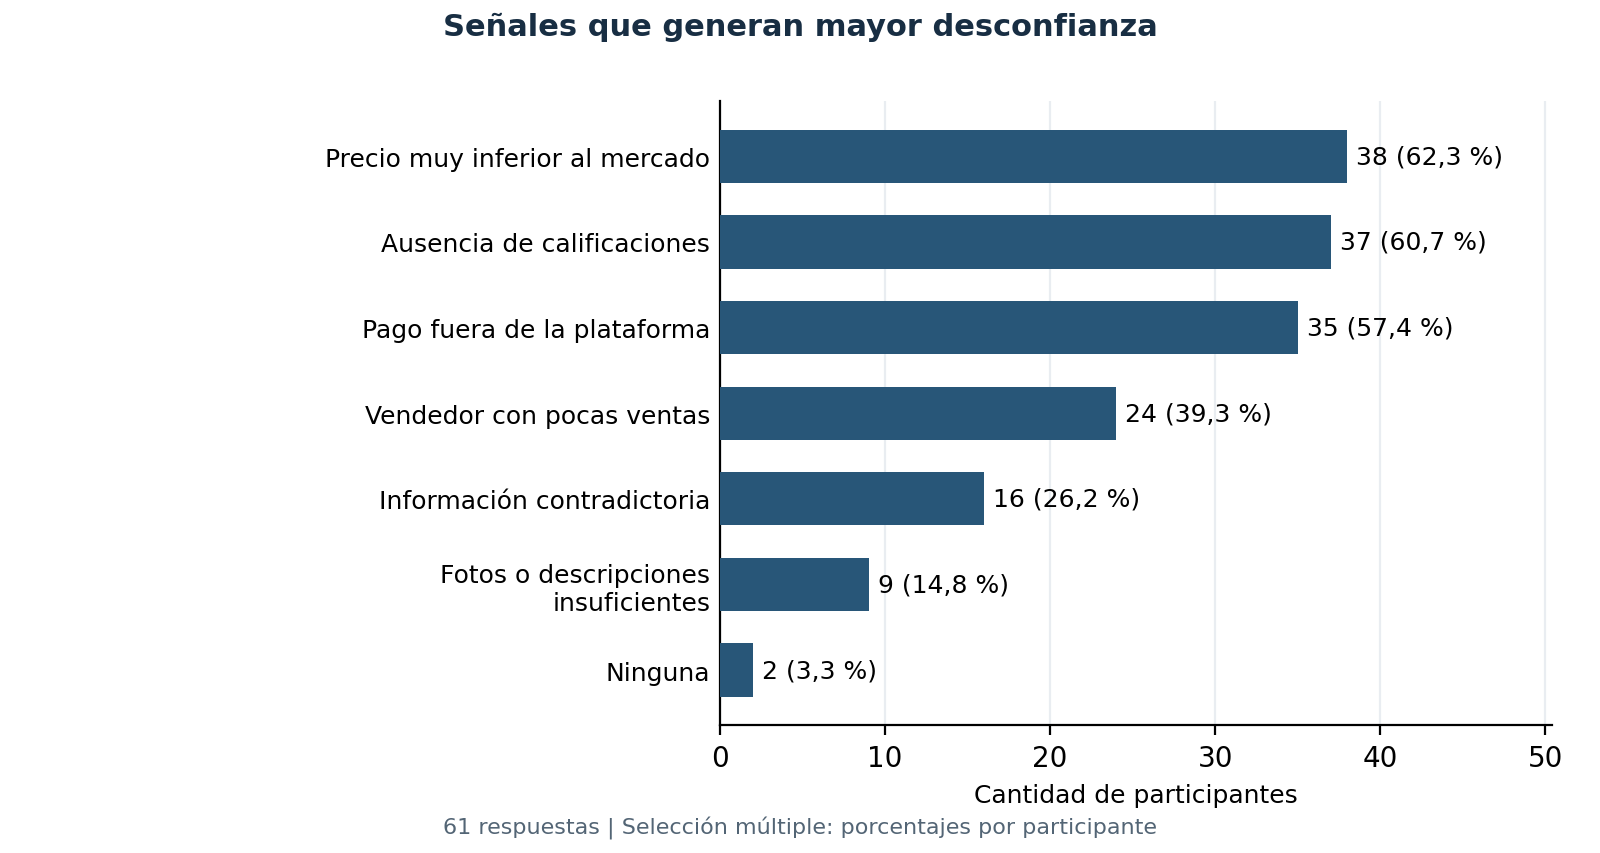
\includegraphics[width=0.94\textwidth,height=0.37\textheight,keepaspectratio]{figuras/marketlens/encuesta/pregunta_07.png}
\caption{Características de publicaciones que generan mayor desconfianza (n=61).}\label{fig:ml-encuesta-07}
\end{figure}

\begin{figure}[H]
\centering
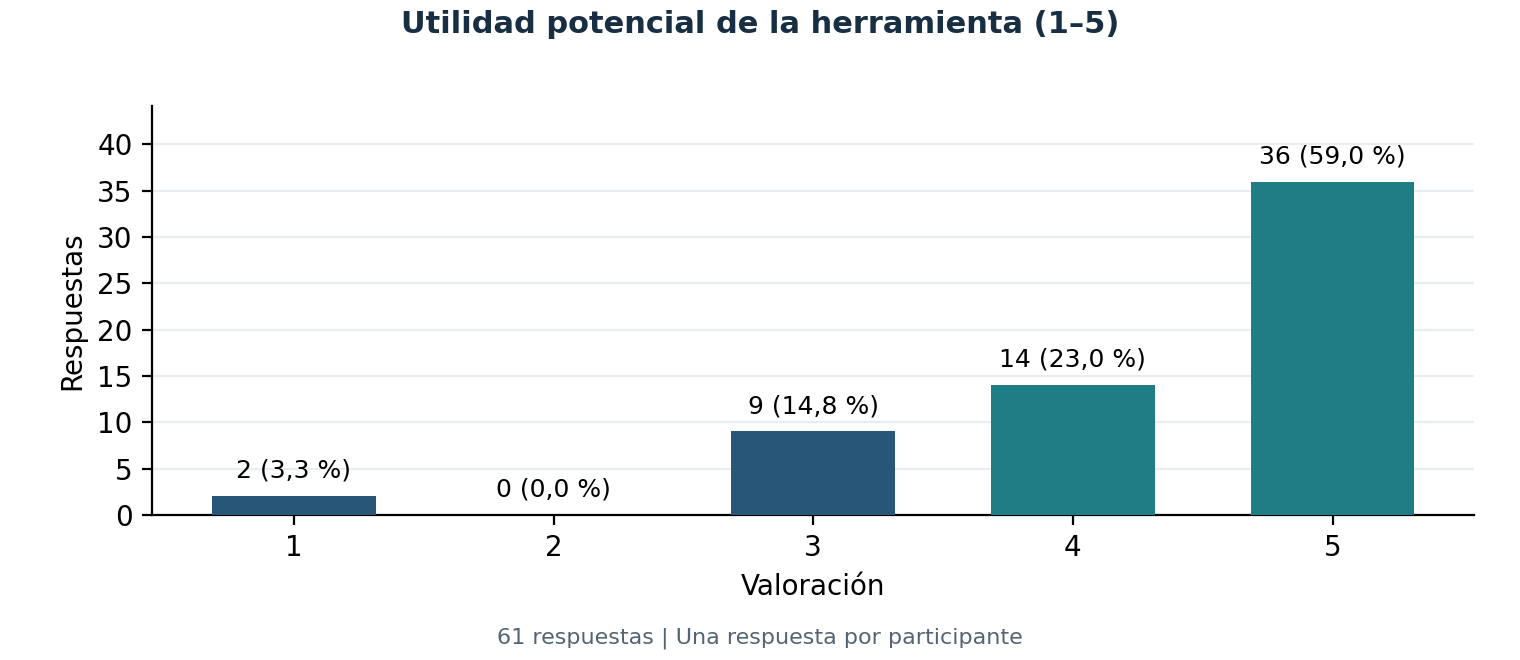
\includegraphics[width=0.94\textwidth,height=0.37\textheight,keepaspectratio]{figuras/marketlens/encuesta/pregunta_08.png}
\caption{Utilidad potencial atribuida a una herramienta de análisis preventivo (n=61).}\label{fig:ml-encuesta-08}
\end{figure}

\begin{figure}[H]
\centering
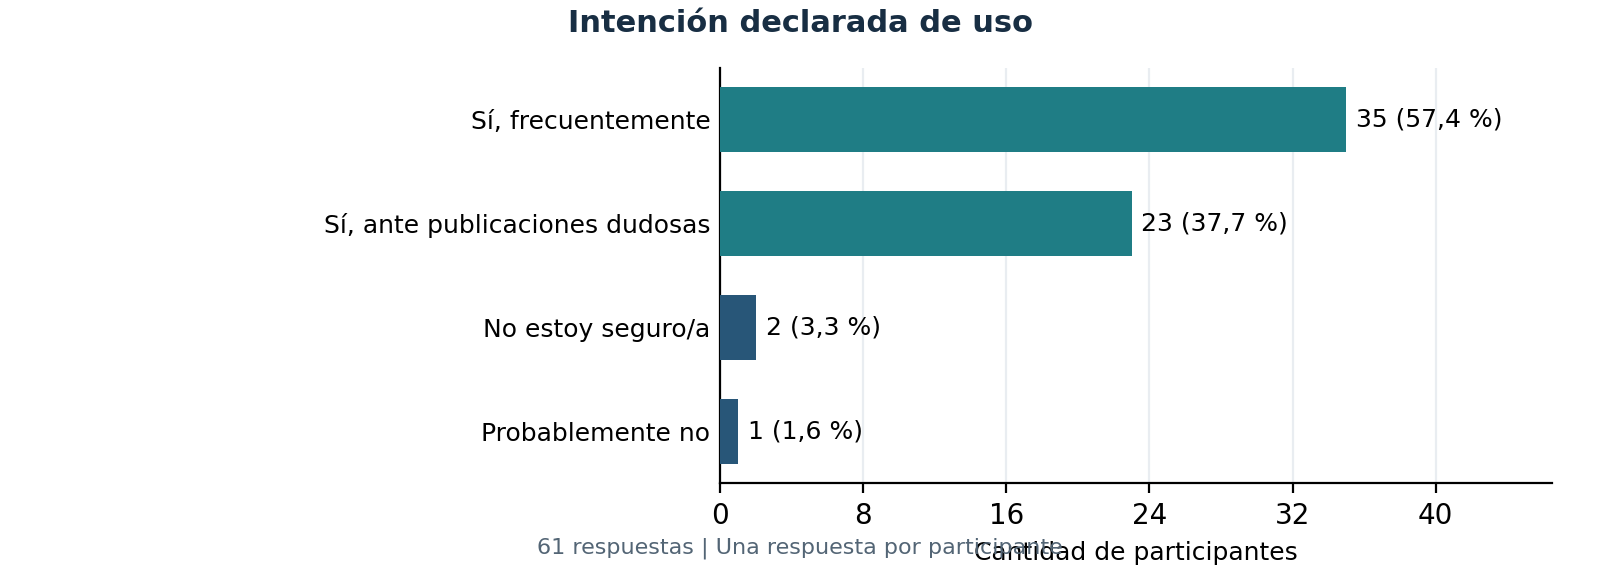
\includegraphics[width=0.94\textwidth,height=0.37\textheight,keepaspectratio]{figuras/marketlens/encuesta/pregunta_09.png}
\caption{Intención declarada de utilización de una herramienta gratuita como la propuesta (n=61).}\label{fig:ml-encuesta-09}
\end{figure}

\begin{figure}[H]
\centering
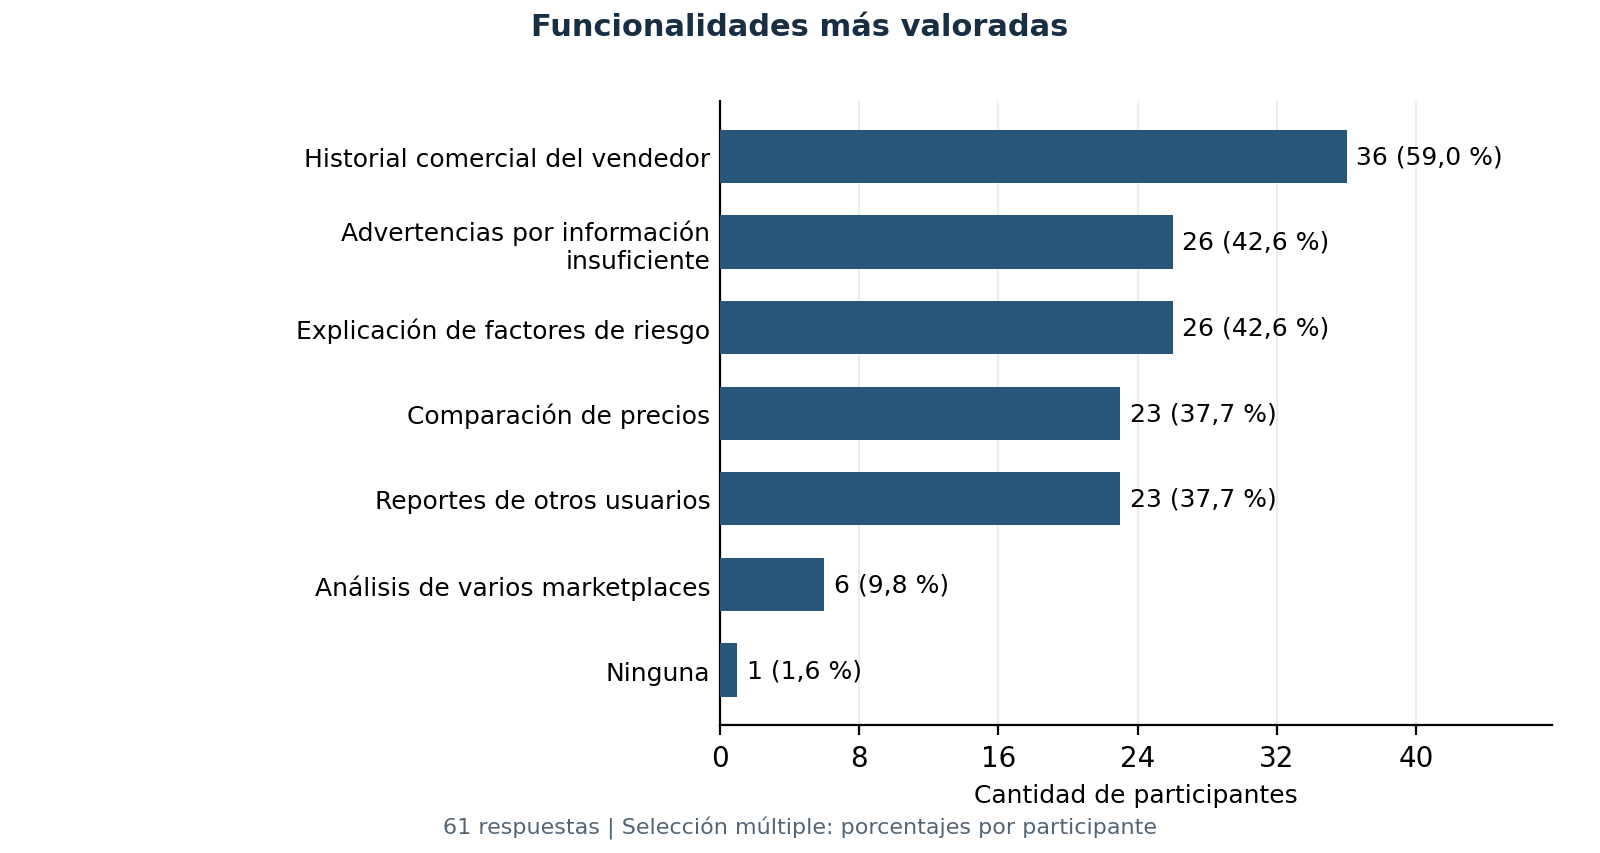
\includegraphics[width=0.94\textwidth,height=0.37\textheight,keepaspectratio]{figuras/marketlens/encuesta/pregunta_10.png}
\caption{Funcionalidades prioritarias para una herramienta de análisis preventivo (n=61).}\label{fig:ml-encuesta-10}
\end{figure}

\begin{figure}[H]
\centering
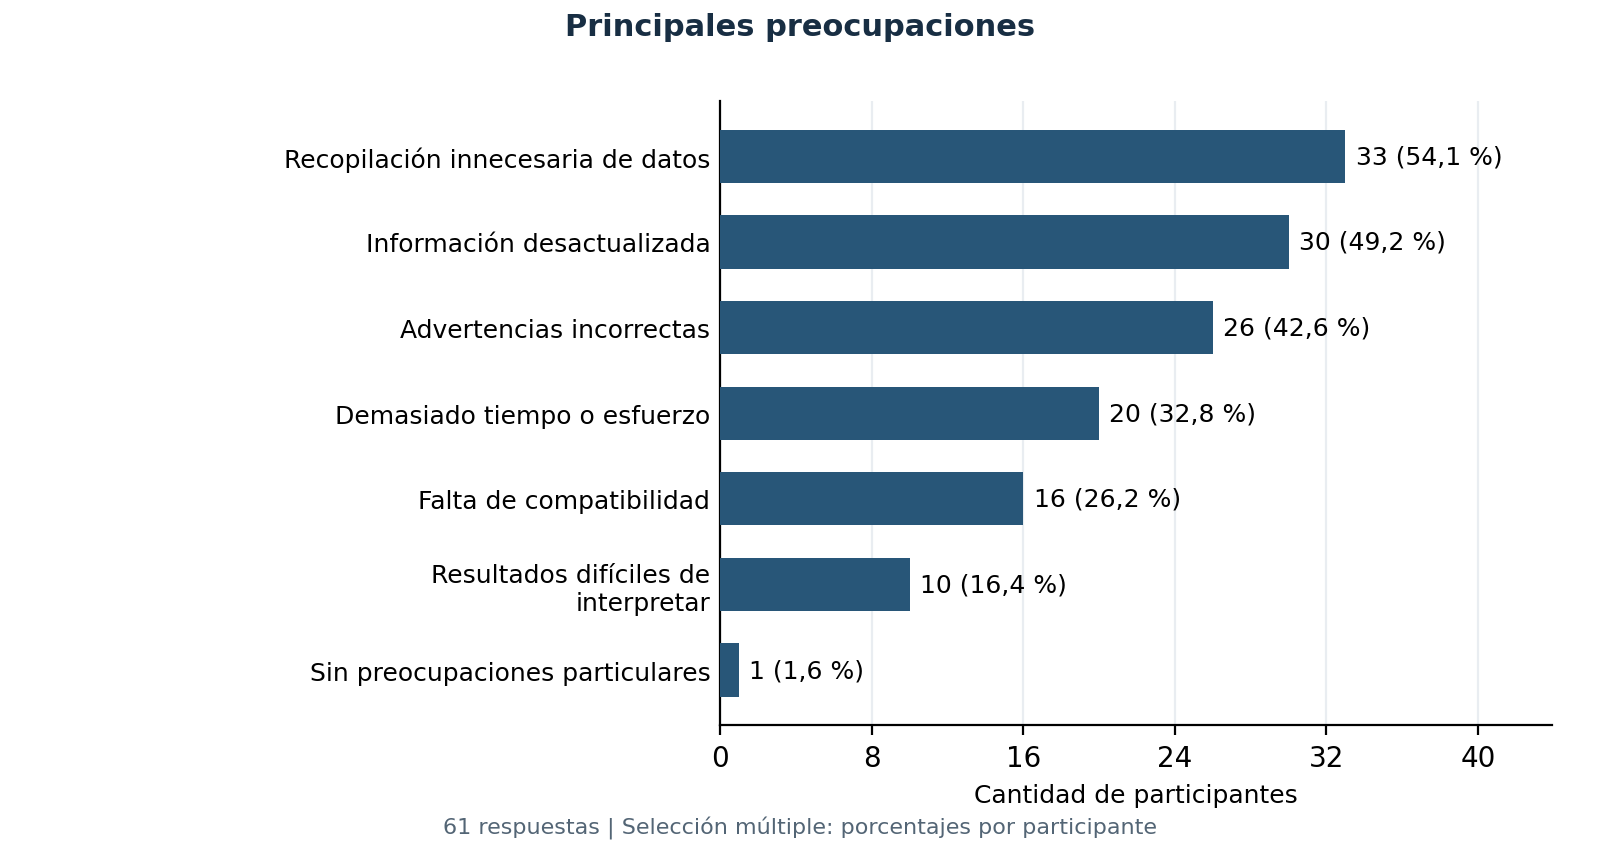
\includegraphics[width=0.94\textwidth,height=0.37\textheight,keepaspectratio]{figuras/marketlens/encuesta/pregunta_11.png}
\caption{Principales preocupaciones respecto del uso de la herramienta (n=61).}\label{fig:ml-encuesta-11}
\end{figure}



\section{Resultados de la encuesta exploratoria}
\label{sec:ml-resultados-encuesta}

Con el propósito de explorar las percepciones de los compradores sobre la seguridad en plataformas digitales y el interés por herramientas preventivas, se aplicó un cuestionario de once preguntas cerradas. El corte de resultados analizado comprende \textbf{61 respuestas} registradas entre el \textbf{10 y el 15 de noviembre de 2026}. El instrumento, sus opciones y las condiciones del relevamiento se incluyen en el apéndice~\ref{apx:encuesta}; el procedimiento se describe en la sección~\ref{subsec:ml-encuesta-metodo}.

La encuesta se difundió mediante contactos del autor y constituye un \textbf{relevamiento exploratorio no probabilístico}. Las cifras expresan percepciones e intenciones declaradas del grupo consultado, sin representatividad estadística de la población general ni evidencia directa de eficacia del motor de detección de fraudes. Las preguntas de selección múltiple admitieron varias alternativas; sus porcentajes se calcularon sobre los 61 participantes y pueden sumar más del 100\,\%.

\begin{table}[H]
\centering
\caption{Síntesis de resultados de la encuesta exploratoria (n=61)}
\label{tab:ml-encuesta-principales}
\small
\begin{tabularx}{\textwidth}{L r r}
\toprule
\tb{Indicador declarado} & \tb{Respuestas} & \tb{Porcentaje} \\
\midrule
Encontró alguna publicación sospechosa & 44/61 & 72,1\,\% \\
Desistió de una compra por desconfianza & 47/61 & 77,0\,\% \\
Calificó la utilidad potencial con 4 o 5 (escala de 1 a 5) & 50/61 & 82,0\,\% \\
Consideraría utilizarla de forma frecuente o ante dudas & 58/61 & 95,1\,\% \\
Asignó 4 o 5 de confianza a los mecanismos actuales & 35/61 & 57,4\,\% \\
\bottomrule
\end{tabularx}
\end{table}

\subsection{Experiencia de compra y criterios de evaluación}

El cuestionario contempló tanto participantes que habían comprado durante los últimos doce meses como otros que no lo habían hecho. El uso de cada plataforma, que podía informarse en conjunto con otras, se presenta en la figura~\ref{fig:ml-encuesta-02}. Mercado Libre fue seleccionado por \textbf{52 personas (85,2\,\%)}. En cuanto a los criterios consultados, los más frecuentes fueron la reputación o calificaciones del vendedor (\textbf{50/61}) y las opiniones de compradores anteriores (\textbf{47/61}), tal como muestra la figura~\ref{fig:ml-encuesta-03}.

\subsection{Percepción de riesgo y confianza}

\textbf{44 participantes (72,1\,\%)} señalaron haber encontrado alguna publicación potencialmente sospechosa (figura~\ref{fig:ml-encuesta-04}), mientras que \textbf{47 (77,0\,\%)} indicaron haber desistido de una compra por desconfianza (figura~\ref{fig:ml-encuesta-05}). Ambas preguntas recogen experiencias autopercibidas: no identifican ni verifican casos reales de fraude.

La confianza en los mecanismos actuales de seguridad y reputación se distribuyó en la escala de 1 a 5, con 35 respuestas en los valores 4 o 5 (\textbf{57,4\,\%}). Entre las características que generaron mayor desconfianza se destacaron el precio considerablemente inferior al de ofertas comparables (\textbf{38 respuestas}), la ausencia de calificaciones u opiniones (\textbf{37}) y la solicitud de pago fuera de la plataforma (\textbf{35}). Se trata de percepciones de los participantes y no de una validación de esos indicadores como predictores de fraude.

\subsection{Utilidad percibida e intención declarada de uso}

Tras presentar una descripción conceptual de una herramienta independiente de análisis preventivo, \textbf{50 participantes (82,0\,\%)} asignaron una utilidad de 4 o 5 en una escala de cinco puntos (figura~\ref{fig:ml-encuesta-08}). Además, \textbf{58 (95,1\,\%)} manifestaron que probablemente utilizarían una herramienta gratuita con frecuencia o ante publicaciones que les generaran dudas (figura~\ref{fig:ml-encuesta-09}). Estas respuestas sugieren \emph{interés declarado} y no constituyen evidencia de adopción efectiva.

En cuanto a funcionalidades, la opción más señalada fue la información sobre el historial comercial del vendedor (\textbf{36 respuestas; 59,0\,\%}). Las advertencias sobre datos insuficientes y la explicación de los factores de riesgo reunieron 26 selecciones cada una. Entre las preocupaciones, destacaron la recopilación innecesaria de datos personales (\textbf{33 respuestas}), la información desactualizada (\textbf{30}) y las advertencias incorrectas (\textbf{26}). Estos resultados sirven para orientar prioridades de transparencia, privacidad y calidad de datos, pero por sí solos no validan decisiones técnicas específicas.

\subsection{Alcance y limitaciones del relevamiento}

La distribución del formulario entre contactos y la participación voluntaria introducen posibles \textbf{sesgos de selección y autoselección}. El instrumento no relevó variables sociodemográficas ni verificó en forma independiente las experiencias declaradas. Por consiguiente, no es posible generalizar los resultados a la totalidad de compradores ni estimar márgenes de error de muestreo probabilístico. Asimismo, la descripción conceptual de MarketLens puede influir en las valoraciones de utilidad e intención de uso.

Estas evidencias complementan la justificación del problema abordado y permiten identificar prioridades expresadas por las personas encuestadas. No deben confundirse con pruebas de usabilidad del prototipo, validaciones de precisión del índice de riesgo o una medición de su impacto real en la prevención de estafas. El presente corte corresponde a 61 respuestas; de incorporarse nuevas respuestas, deben recalcularse todos los porcentajes y sustituirse los gráficos correspondientes.

\subsection{Distribución completa de respuestas}

Las figuras siguientes presentan las frecuencias absolutas y los porcentajes observados para las once preguntas, incluida la opción de valoración no seleccionada en las escalas. En preguntas de selección múltiple, el denominador continúa siendo el número total de participantes (61).
\begin{figure}[H]
\centering
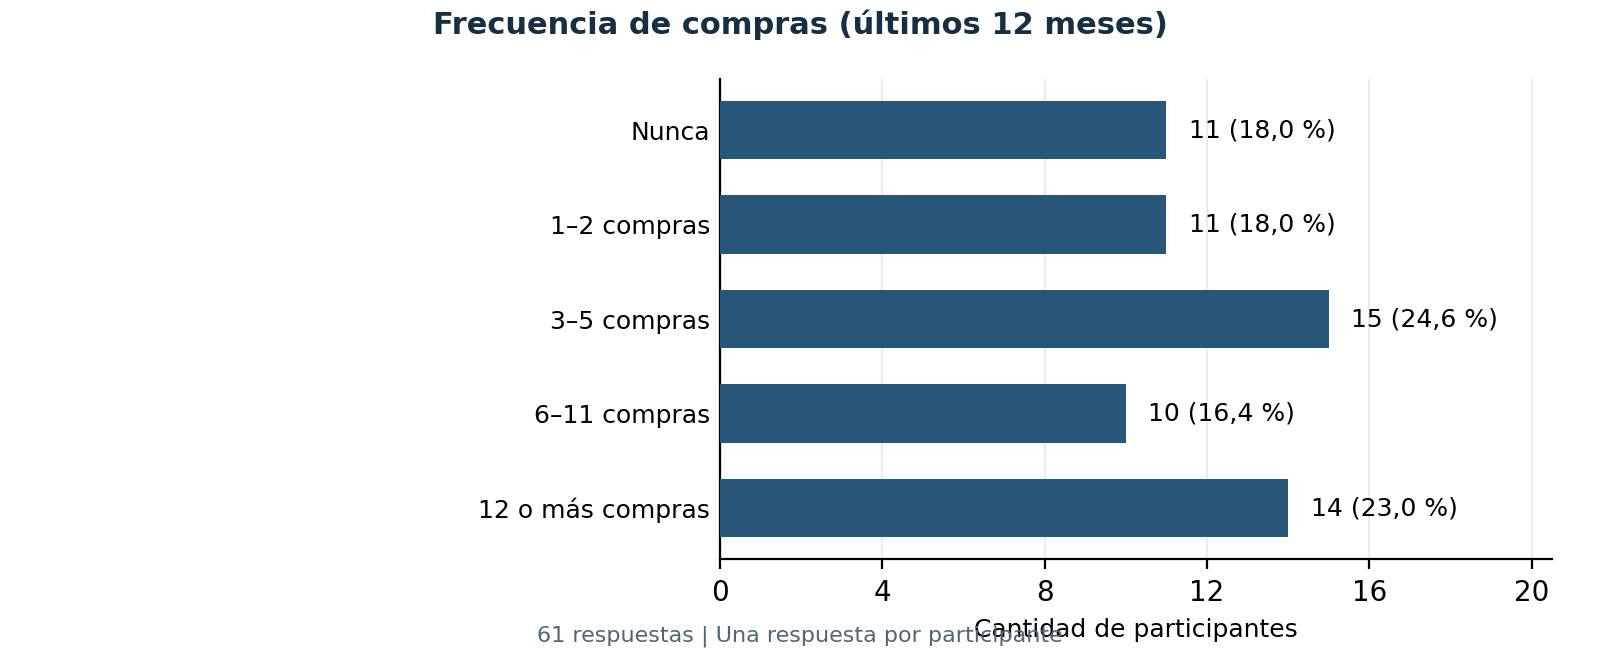
\includegraphics[width=0.94\textwidth,height=0.37\textheight,keepaspectratio]{figuras/marketlens/encuesta/pregunta_01.png}
\caption{Frecuencia de compra declarada en marketplaces durante los últimos doce meses (n=61).}\label{fig:ml-encuesta-01}
\end{figure}

\begin{figure}[H]
\centering
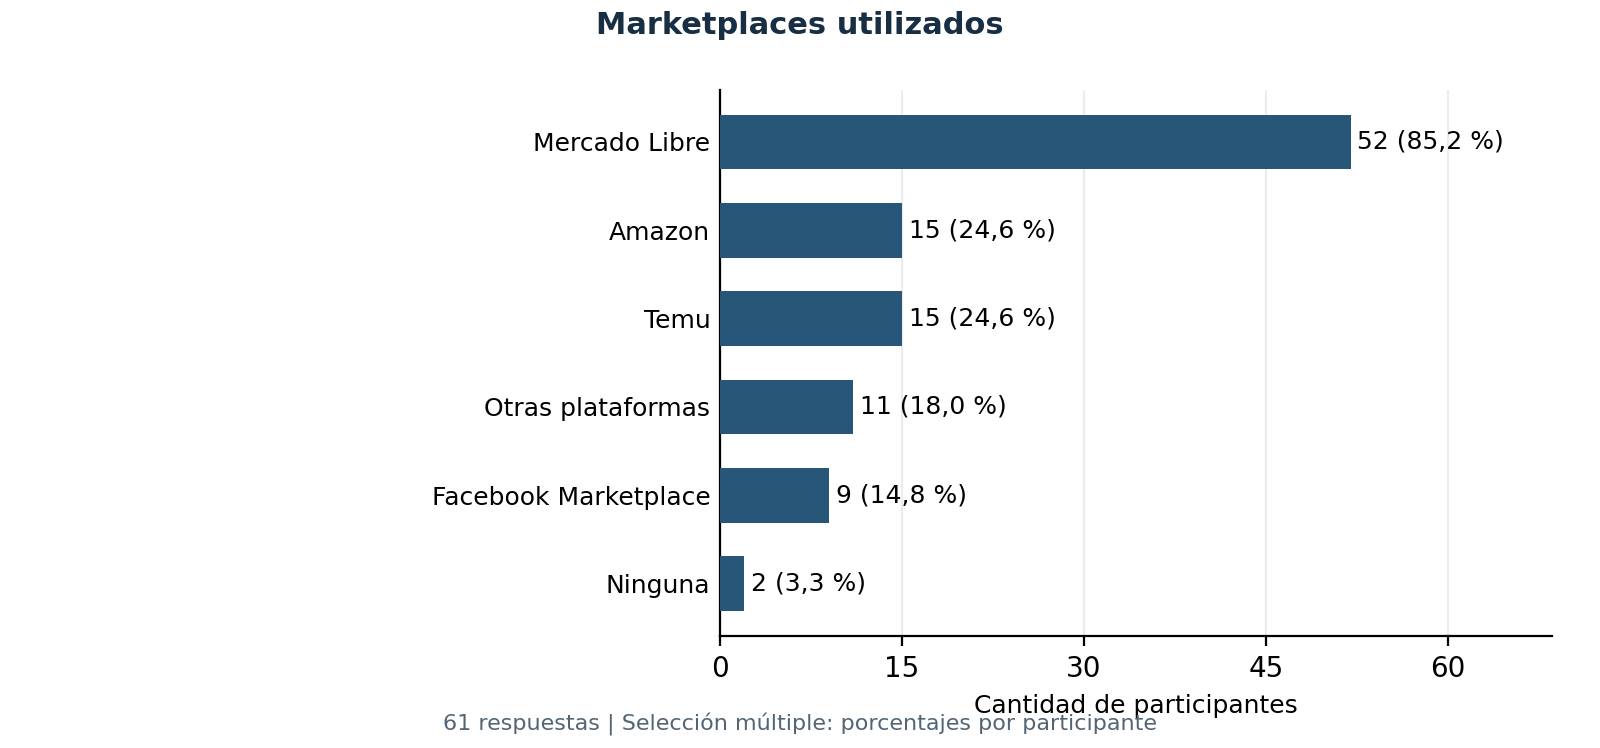
\includegraphics[width=0.94\textwidth,height=0.37\textheight,keepaspectratio]{figuras/marketlens/encuesta/pregunta_02.png}
\caption{Plataformas utilizadas por los encuestados durante los últimos doce meses (n=61).}\label{fig:ml-encuesta-02}
\end{figure}

\begin{figure}[H]
\centering
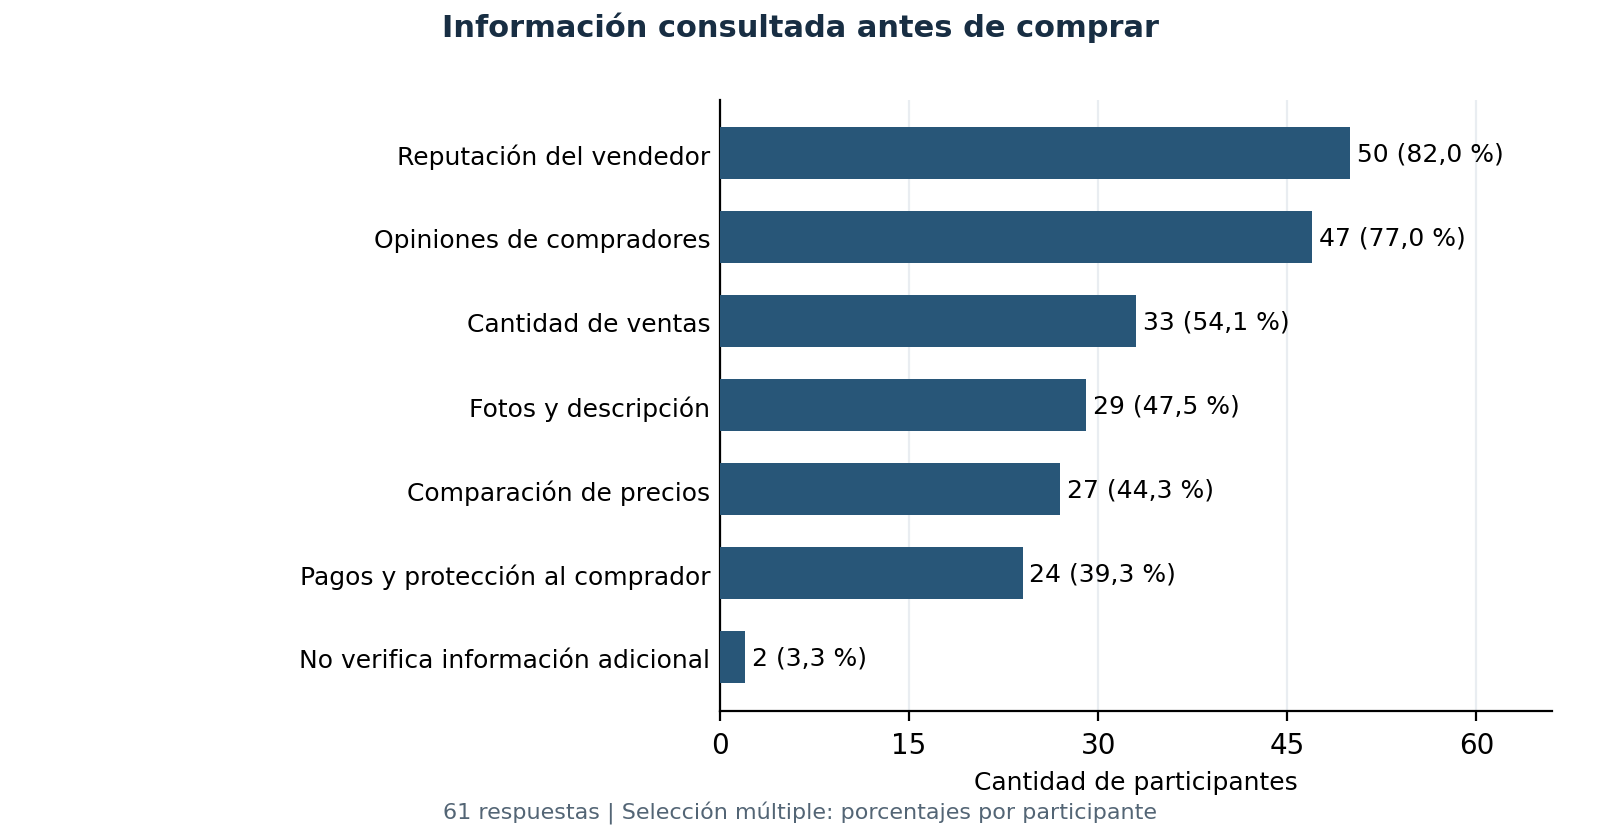
\includegraphics[width=0.94\textwidth,height=0.37\textheight,keepaspectratio]{figuras/marketlens/encuesta/pregunta_03.png}
\caption{Información habitualmente consultada para evaluar publicaciones o vendedores (n=61).}\label{fig:ml-encuesta-03}
\end{figure}

\begin{figure}[H]
\centering
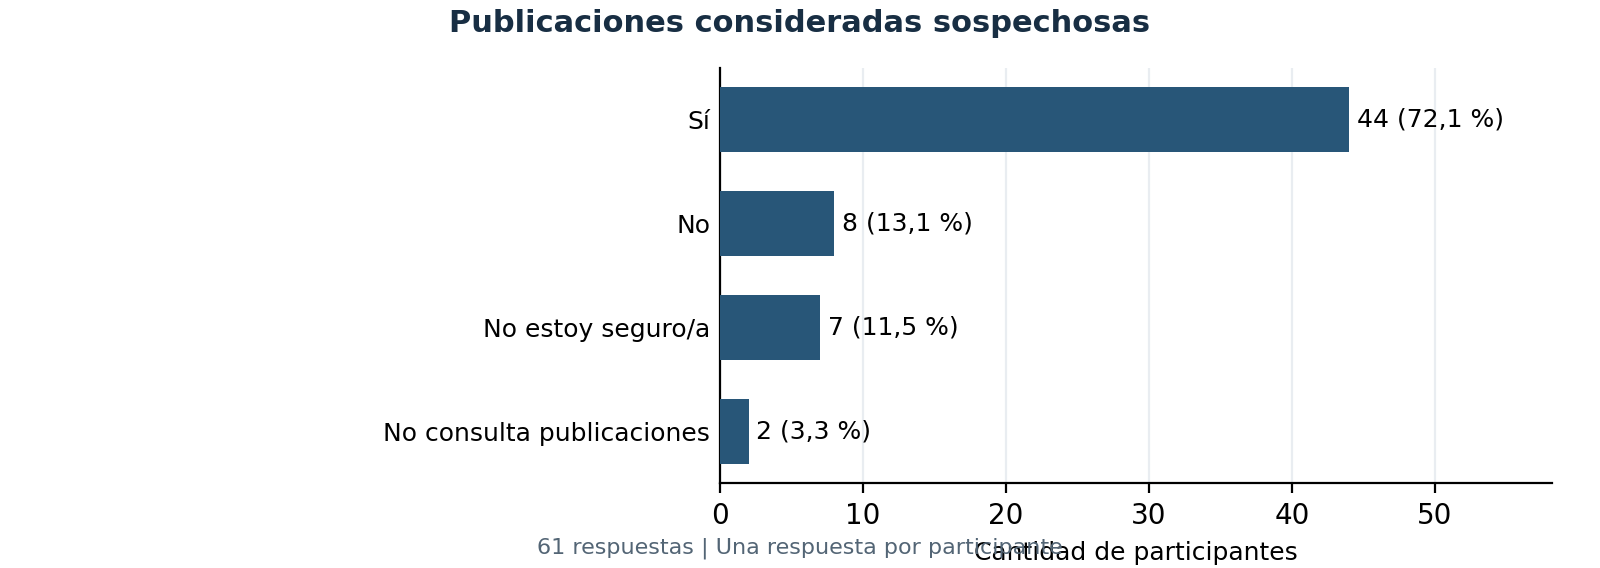
\includegraphics[width=0.94\textwidth,height=0.37\textheight,keepaspectratio]{figuras/marketlens/encuesta/pregunta_04.png}
\caption{Encuestados que identificaron publicaciones potencialmente sospechosas (n=61).}\label{fig:ml-encuesta-04}
\end{figure}

\begin{figure}[H]
\centering
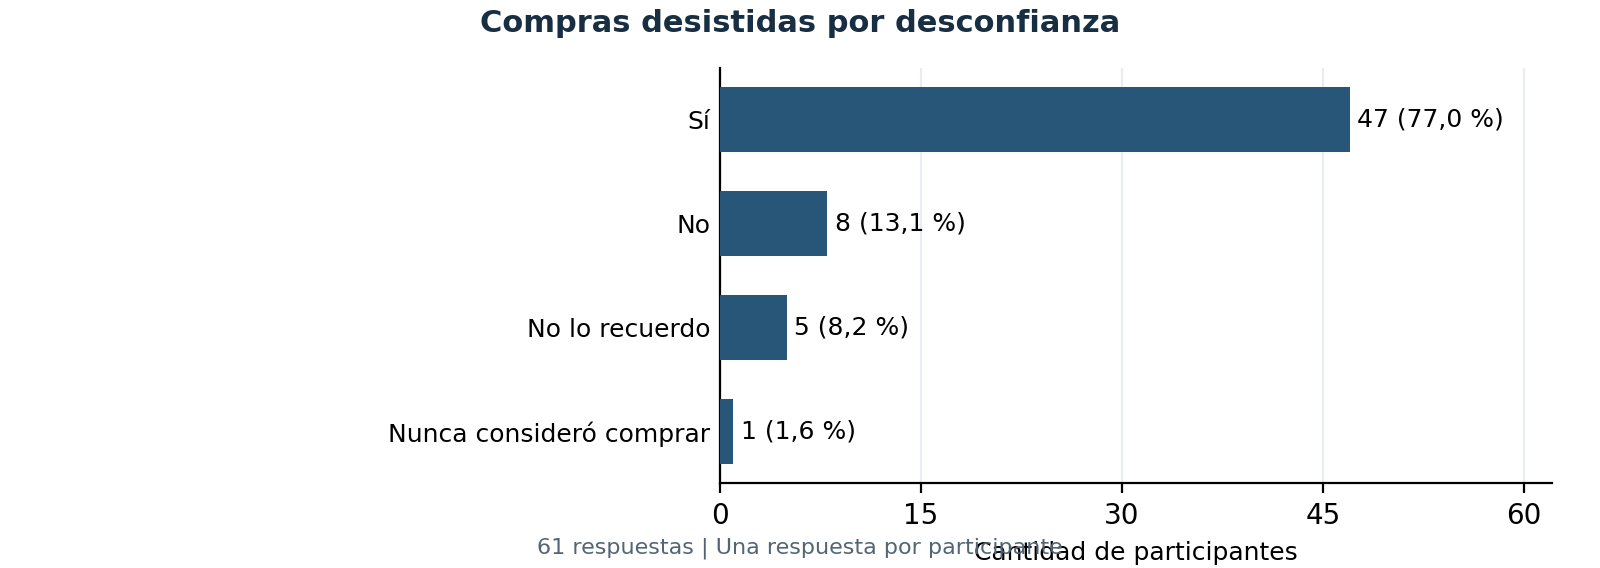
\includegraphics[width=0.94\textwidth,height=0.37\textheight,keepaspectratio]{figuras/marketlens/encuesta/pregunta_05.png}
\caption{Encuestados que desistieron de una compra por desconfianza (n=61).}\label{fig:ml-encuesta-05}
\end{figure}

\begin{figure}[H]
\centering
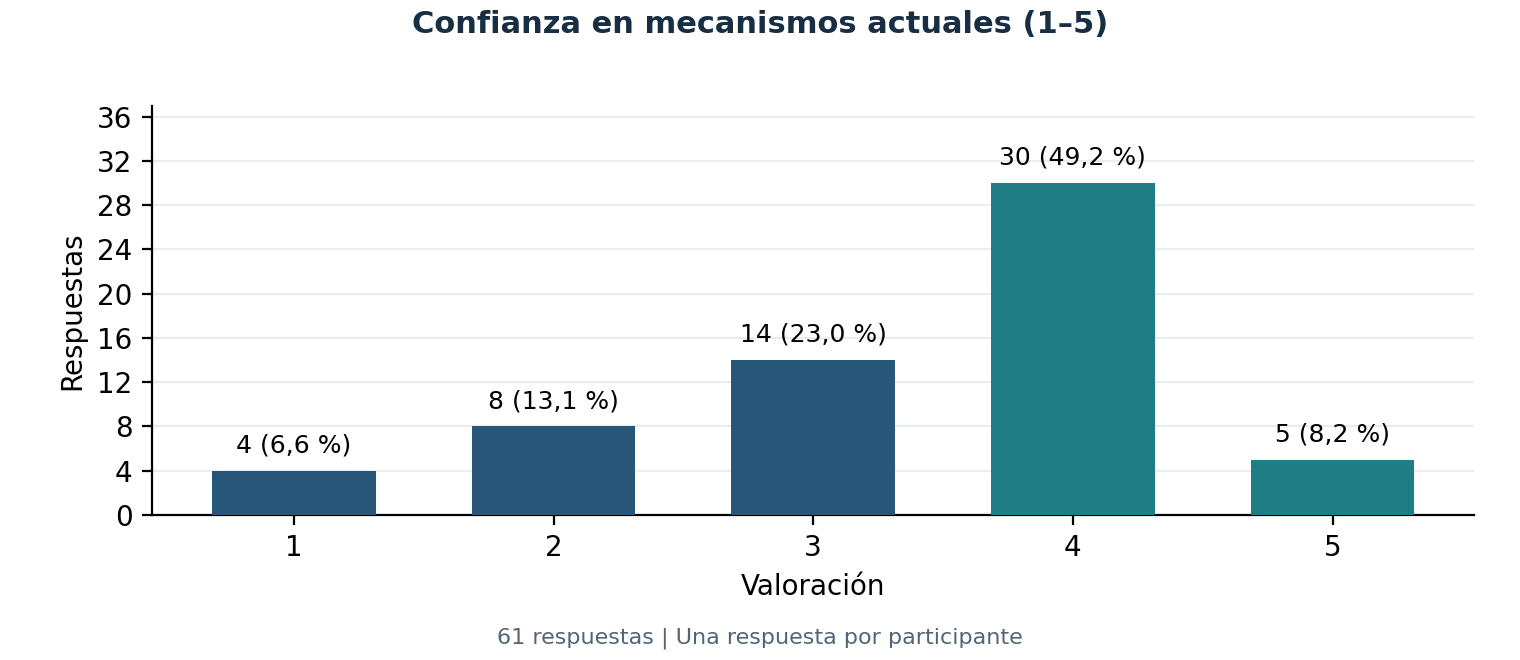
\includegraphics[width=0.94\textwidth,height=0.37\textheight,keepaspectratio]{figuras/marketlens/encuesta/pregunta_06.png}
\caption{Confianza declarada en los mecanismos actuales de seguridad y reputación (n=61).}\label{fig:ml-encuesta-06}
\end{figure}

\begin{figure}[H]
\centering
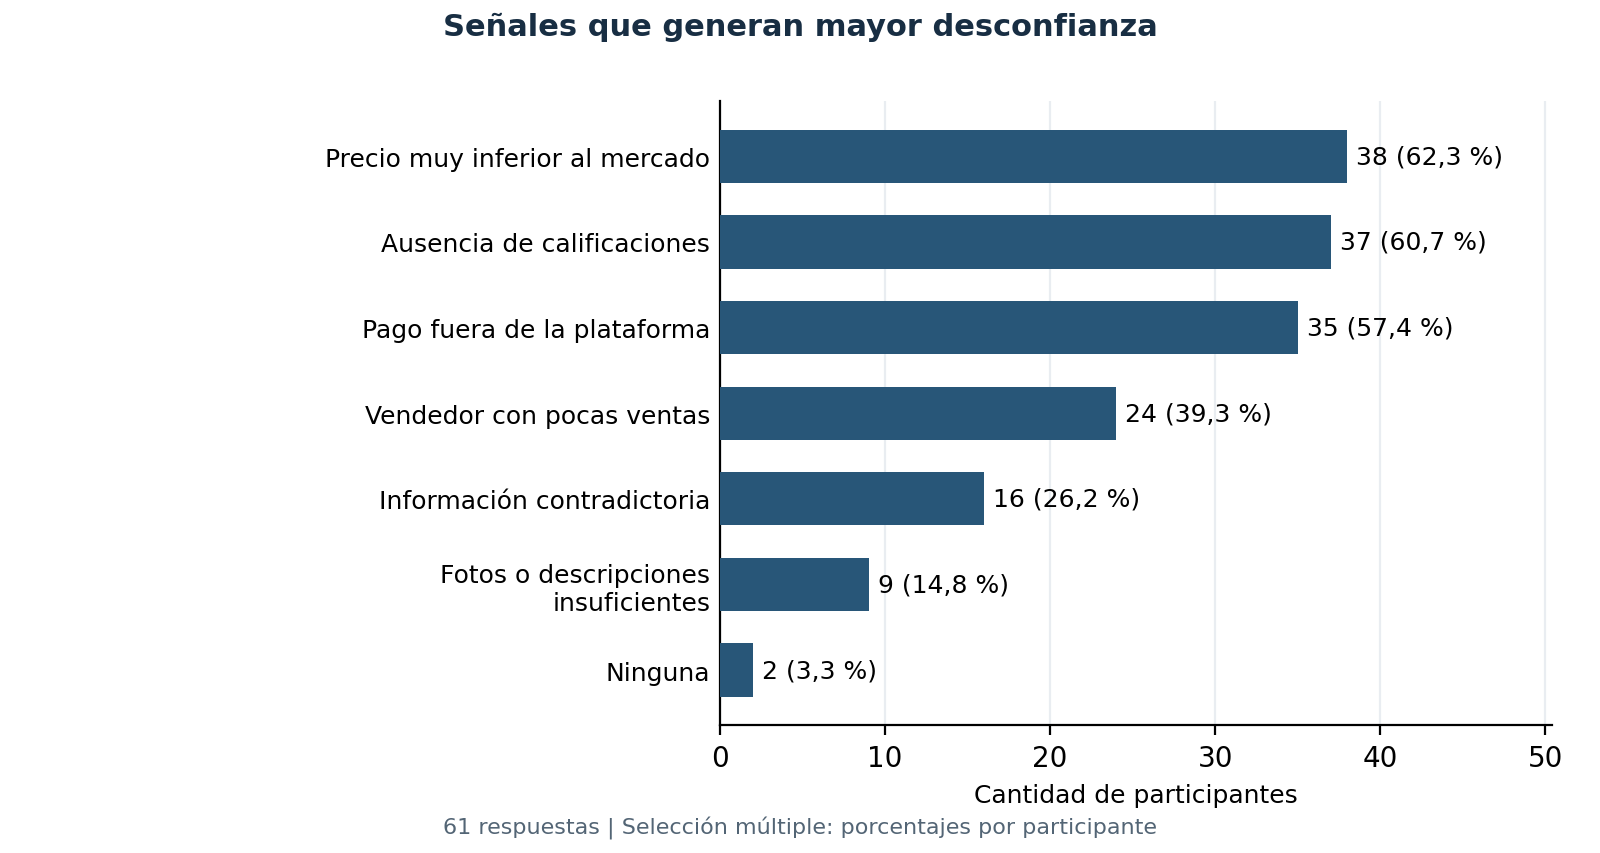
\includegraphics[width=0.94\textwidth,height=0.37\textheight,keepaspectratio]{figuras/marketlens/encuesta/pregunta_07.png}
\caption{Características de publicaciones que generan mayor desconfianza (n=61).}\label{fig:ml-encuesta-07}
\end{figure}

\begin{figure}[H]
\centering
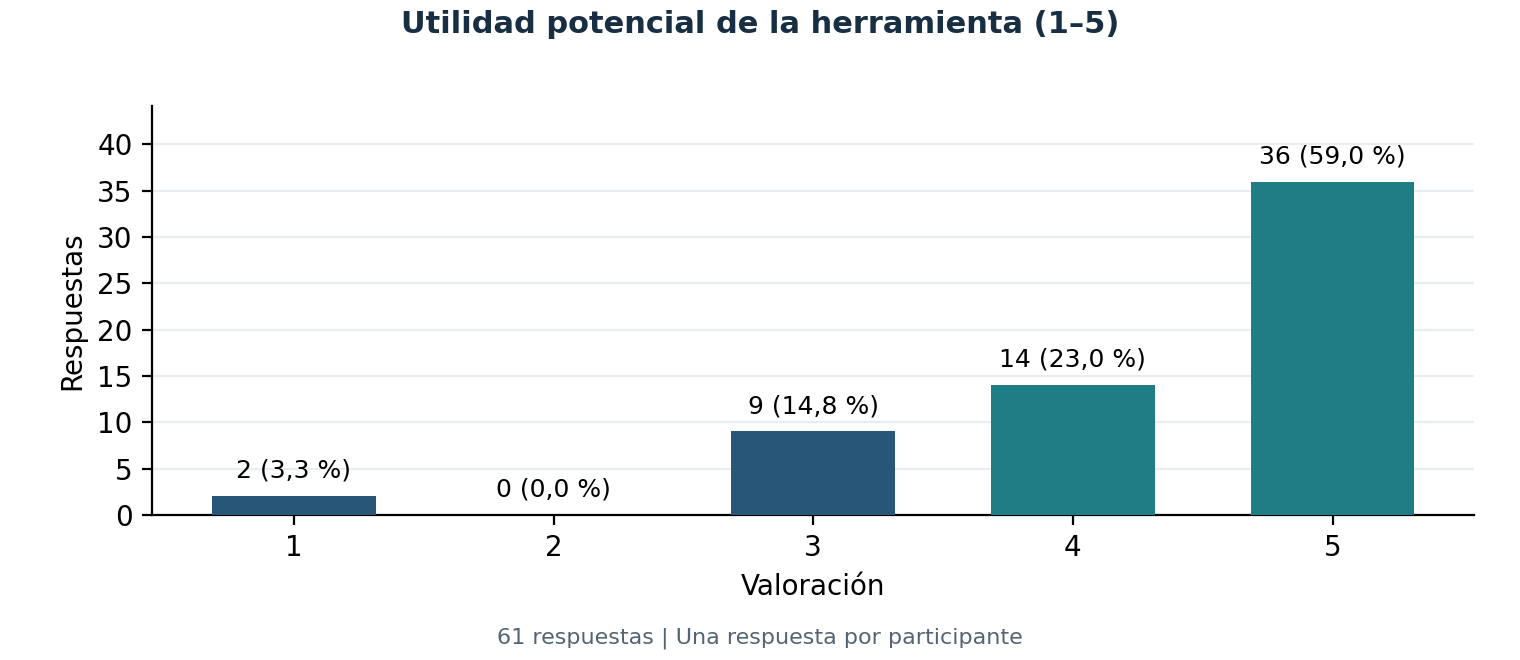
\includegraphics[width=0.94\textwidth,height=0.37\textheight,keepaspectratio]{figuras/marketlens/encuesta/pregunta_08.png}
\caption{Utilidad potencial atribuida a una herramienta de análisis preventivo (n=61).}\label{fig:ml-encuesta-08}
\end{figure}

\begin{figure}[H]
\centering
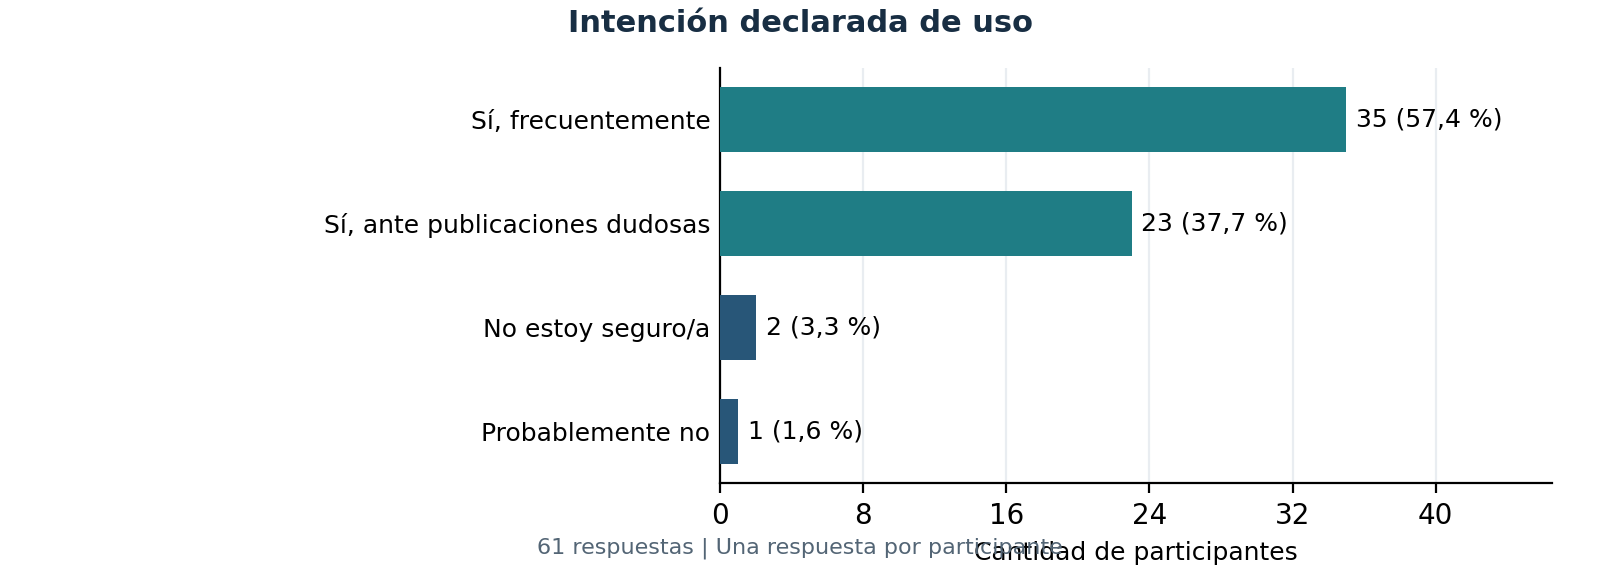
\includegraphics[width=0.94\textwidth,height=0.37\textheight,keepaspectratio]{figuras/marketlens/encuesta/pregunta_09.png}
\caption{Intención declarada de utilización de una herramienta gratuita como la propuesta (n=61).}\label{fig:ml-encuesta-09}
\end{figure}

\begin{figure}[H]
\centering
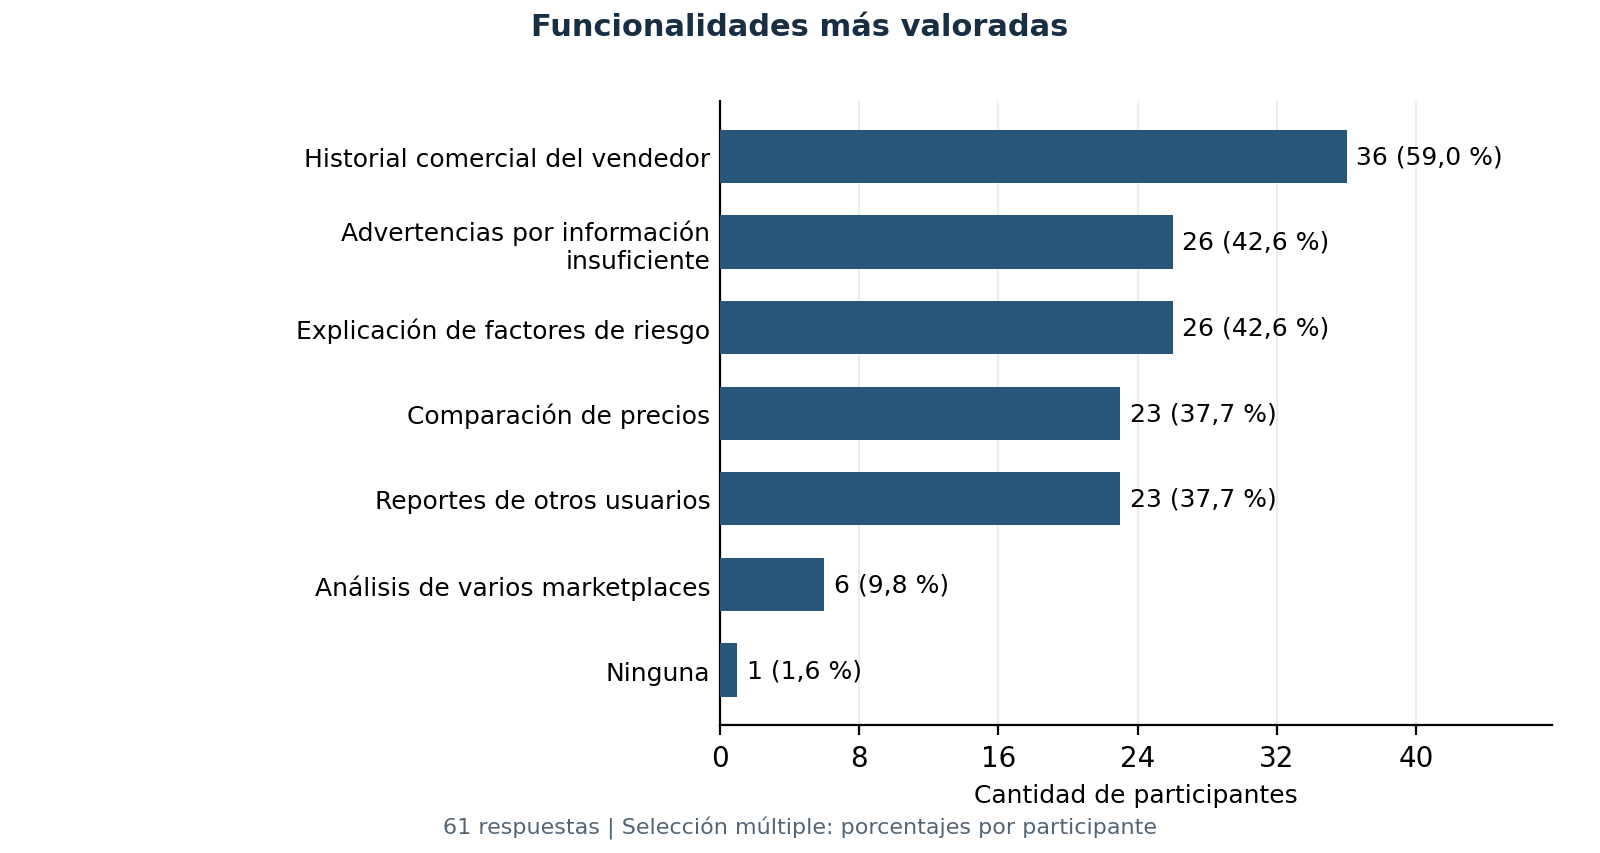
\includegraphics[width=0.94\textwidth,height=0.37\textheight,keepaspectratio]{figuras/marketlens/encuesta/pregunta_10.png}
\caption{Funcionalidades prioritarias para una herramienta de análisis preventivo (n=61).}\label{fig:ml-encuesta-10}
\end{figure}

\begin{figure}[H]
\centering
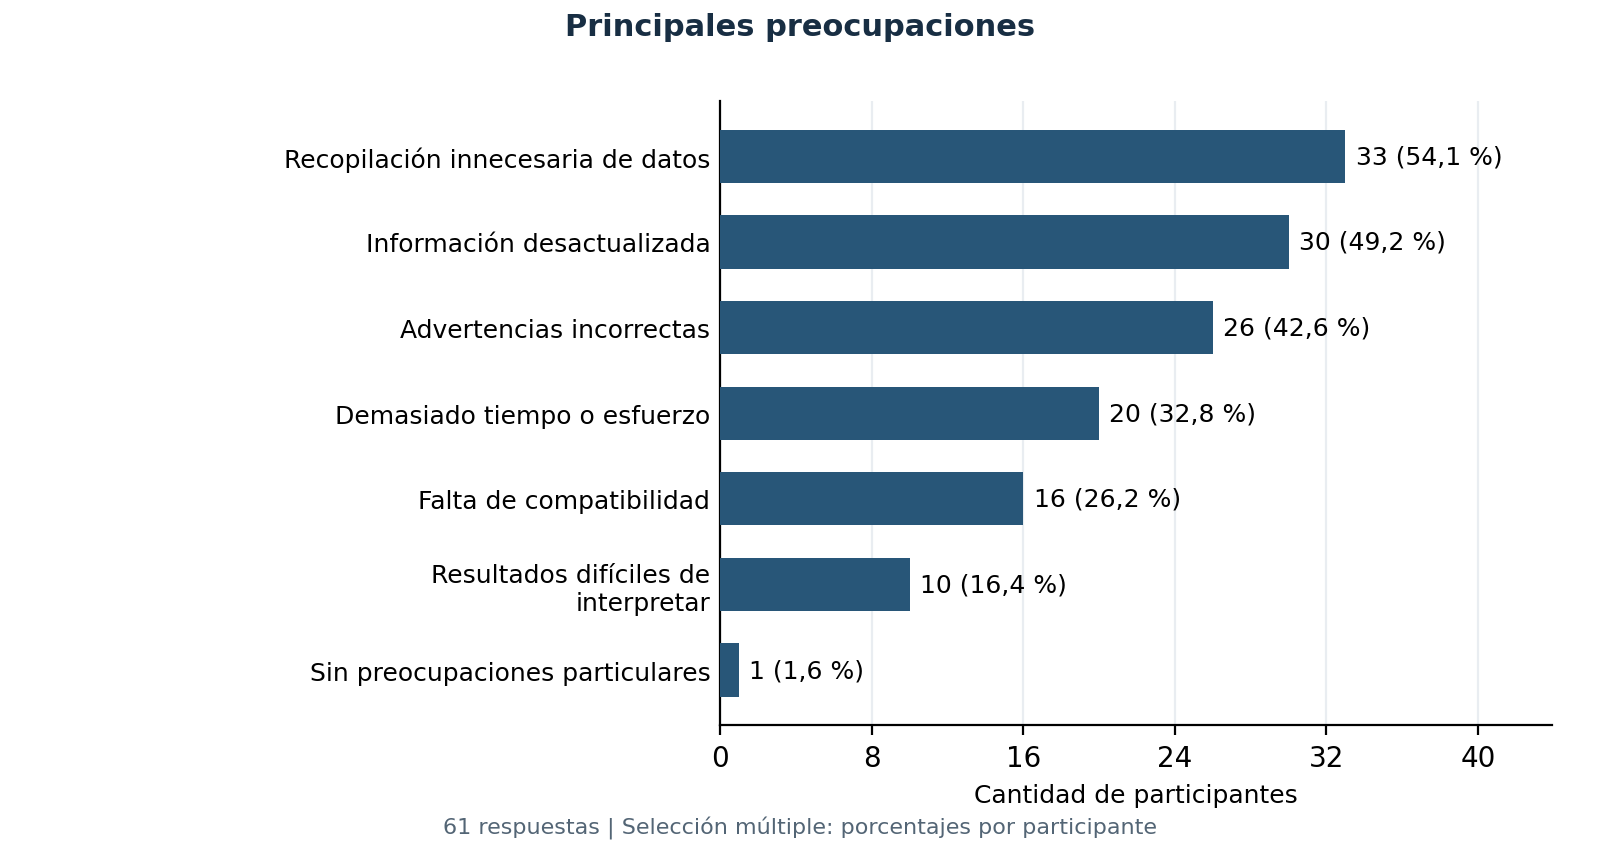
\includegraphics[width=0.94\textwidth,height=0.37\textheight,keepaspectratio]{figuras/marketlens/encuesta/pregunta_11.png}
\caption{Principales preocupaciones respecto del uso de la herramienta (n=61).}\label{fig:ml-encuesta-11}
\end{figure}


